
%% bare_conf.tex
%% V1.3
%% 2007/01/11
%% by Michael Shell
%% See:
%% http://www.michaelshell.org/
%% for current contact information.
%%
%% This is a skeleton file demonstrating the use of IEEEtran.cls
%% (requires IEEEtran.cls version 1.7 or later) with an IEEE conference paper.
%%
%% Support sites:
%% http://www.michaelshell.org/tex/ieeetran/
%% http://www.ctan.org/tex-archive/macros/latex/contrib/IEEEtran/
%% and
%% http://www.ieee.org/

%%*************************************************************************
%% Legal Notice:
%% This code is offered as-is without any warranty either expressed or
%% implied; without even the implied warranty of MERCHANTABILITY or
%% FITNESS FOR A PARTICULAR PURPOSE! 
%% User assumes all risk.
%% In no event shall IEEE or any contributor to this code be liable for
%% any damages or losses, including, but not limited to, incidental,
%% consequential, or any other damages, resulting from the use or misuse
%% of any information contained here.
%%
%% All comments are the opinions of their respective authors and are not
%% necessarily endorsed by the IEEE.
%%
%% This work is distributed under the LaTeX Project Public License (LPPL)
%% ( http://www.latex-project.org/ ) version 1.3, and may be freely used,
%% distributed and modified. A copy of the LPPL, version 1.3, is included
%% in the base LaTeX documentation of all distributions of LaTeX released
%% 2003/12/01 or later.
%% Retain all contribution notices and credits.
%% ** Modified files should be clearly indicated as such, including  **
%% ** renaming them and changing author support contact information. **
%%
%% File list of work: IEEEtran.cls, IEEEtran_HOWTO.pdf, bare_adv.tex,
%%                    bare_conf.tex, bare_jrnl.tex, bare_jrnl_compsoc.tex
%%*************************************************************************

% *** Authors should verify (and, if needed, correct) their LaTeX system  ***
% *** with the testflow diagnostic prior to trusting their LaTeX platform ***
% *** with production work. IEEE's font choices can trigger bugs that do  ***
% *** not appear when using other class files.                            ***
% The testflow support page is at:
% http://www.michaelshell.org/tex/testflow/



% Note that the a4paper option is mainly intended so that authors in
% countries using A4 can easily print to A4 and see how their papers will
% look in print - the typesetting of the document will not typically be
% affected with changes in paper size (but the bottom and side margins will).
% Use the testflow package mentioned above to verify correct handling of
% both paper sizes by the user's LaTeX system.
%
% Also note that the "draftcls" or "draftclsnofoot", not "draft", option
% should be used if it is desired that the figures are to be displayed in
% draft mode.
%
\documentclass[conference]{IEEEtran}
% Add the compsoc option for Computer Society conferences.
%
% If IEEEtran.cls has not been installed into the LaTeX system files,
% manually specify the path to it like:
% \documentclass[conference]{../sty/IEEEtran}





% Some very useful LaTeX packages include:
% (uncomment the ones you want to load)


% *** MISC UTILITY PACKAGES ***
%
%\usepackage{ifpdf}
% Heiko Oberdiek's ifpdf.sty is very useful if you need conditional
% compilation based on whether the output is pdf or dvi.
% usage:
% \ifpdf
%   % pdf code
% \else
%   % dvi code
% \fi
% The latest version of ifpdf.sty can be obtained from:
% http://www.ctan.org/tex-archive/macros/latex/contrib/oberdiek/
% Also, note that IEEEtran.cls V1.7 and later provides a builtin
% \ifCLASSINFOpdf conditional that works the same way.
% When switching from latex to pdflatex and vice-versa, the compiler may
% have to be run twice to clear warning/error messages.






% *** CITATION PACKAGES ***
%
%\usepackage{cite}
% cite.sty was written by Donald Arseneau
% V1.6 and later of IEEEtran pre-defines the format of the cite.sty package
% \cite{} output to follow that of IEEE. Loading the cite package will
% result in citation numbers being automatically sorted and properly
% "compressed/ranged". e.g., [1], [9], [2], [7], [5], [6] without using
% cite.sty will become [1], [2], [5]--[7], [9] using cite.sty. cite.sty's
% \cite will automatically add leading space, if needed. Use cite.sty's
% noadjust option (cite.sty V3.8 and later) if you want to turn this off.
% cite.sty is already installed on most LaTeX systems. Be sure and use
% version 4.0 (2003-05-27) and later if using hyperref.sty. cite.sty does
% not currently provide for hyperlinked citations.
% The latest version can be obtained at:
% http://www.ctan.org/tex-archive/macros/latex/contrib/cite/
% The documentation is contained in the cite.sty file itself.






% *** GRAPHICS RELATED PACKAGES ***
%
\ifCLASSINFOpdf
   \usepackage[pdftex]{graphicx}
  % declare the path(s) where your graphic files are
  % \graphicspath{{../pdf/}{../jpeg/}}
  % and their extensions so you won't have to specify these with
  % every instance of \includegraphics
  % \DeclareGraphicsExtensions{.pdf,.jpeg,.png}
\else
  % or other class option (dvipsone, dvipdf, if not using dvips). graphicx
  % will default to the driver specified in the system graphics.cfg if no
  % driver is specified.
  % \usepackage[dvips]{graphicx}
  % declare the path(s) where your graphic files are
  % \graphicspath{{../eps/}}
  % and their extensions so you won't have to specify these with
  % every instance of \includegraphics
  % \DeclareGraphicsExtensions{.eps}
\fi
% graphicx was written by David Carlisle and Sebastian Rahtz. It is
% required if you want graphics, photos, etc. graphicx.sty is already
% installed on most LaTeX systems. The latest version and documentation can
% be obtained at: 
% http://www.ctan.org/tex-archive/macros/latex/required/graphics/
% Another good source of documentation is "Using Imported Graphics in
% LaTeX2e" by Keith Reckdahl which can be found as epslatex.ps or
% epslatex.pdf at: http://www.ctan.org/tex-archive/info/
%
% latex, and pdflatex in dvi mode, support graphics in encapsulated
% postscript (.eps) format. pdflatex in pdf mode supports graphics
% in .pdf, .jpeg, .png and .mps (metapost) formats. Users should ensure
% that all non-photo figures use a vector format (.eps, .pdf, .mps) and
% not a bitmapped formats (.jpeg, .png). IEEE frowns on bitmapped formats
% which can result in "jaggedy"/blurry rendering of lines and letters as
% well as large increases in file sizes.
%
% You can find documentation about the pdfTeX application at:
% http://www.tug.org/applications/pdftex

\usepackage{subfigure}



% *** MATH PACKAGES ***
%
\usepackage[cmex10]{amsmath}
% A popular package from the American Mathematical Society that provides
% many useful and powerful commands for dealing with mathematics. If using
% it, be sure to load this package with the cmex10 option to ensure that
% only type 1 fonts will utilized at all point sizes. Without this option,
% it is possible that some math symbols, particularly those within
% footnotes, will be rendered in bitmap form which will result in a
% document that can not be IEEE Xplore compliant!
%
% Also, note that the amsmath package sets \interdisplaylinepenalty to 10000
% thus preventing page breaks from occurring within multiline equations. Use:
%\interdisplaylinepenalty=2500
% after loading amsmath to restore such page breaks as IEEEtran.cls normally
% does. amsmath.sty is already installed on most LaTeX systems. The latest
% version and documentation can be obtained at:
% http://www.ctan.org/tex-archive/macros/latex/required/amslatex/math/





% *** SPECIALIZED LIST PACKAGES ***
%
\usepackage{algorithmic}
% algorithmic.sty was written by Peter Williams and Rogerio Brito.
% This package provides an algorithmic environment fo describing algorithms.
% You can use the algorithmic environment in-text or within a figure
% environment to provide for a floating algorithm. Do NOT use the algorithm
% floating environment provided by algorithm.sty (by the same authors) or
% algorithm2e.sty (by Christophe Fiorio) as IEEE does not use dedicated
% algorithm float types and packages that provide these will not provide
% correct IEEE style captions. The latest version and documentation of
% algorithmic.sty can be obtained at:
% http://www.ctan.org/tex-archive/macros/latex/contrib/algorithms/
% There is also a support site at:
% http://algorithms.berlios.de/index.html
% Also of interest may be the (relatively newer and more customizable)
% algorithmicx.sty package by Szasz Janos:
% http://www.ctan.org/tex-archive/macros/latex/contrib/algorithmicx/




% *** ALIGNMENT PACKAGES ***
%
\usepackage{array}
% Frank Mittelbach's and David Carlisle's array.sty patches and improves
% the standard LaTeX2e array and tabular environments to provide better
% appearance and additional user controls. As the default LaTeX2e table
% generation code is lacking to the point of almost being broken with
% respect to the quality of the end results, all users are strongly
% advised to use an enhanced (at the very least that provided by array.sty)
% set of table tools. array.sty is already installed on most systems. The
% latest version and documentation can be obtained at:
% http://www.ctan.org/tex-archive/macros/latex/required/tools/


%\usepackage{mdwmath}
%\usepackage{mdwtab}
% Also highly recommended is Mark Wooding's extremely powerful MDW tools,
% especially mdwmath.sty and mdwtab.sty which are used to format equations
% and tables, respectively. The MDWtools set is already installed on most
% LaTeX systems. The lastest version and documentation is available at:
% http://www.ctan.org/tex-archive/macros/latex/contrib/mdwtools/


% IEEEtran contains the IEEEeqnarray family of commands that can be used to
% generate multiline equations as well as matrices, tables, etc., of high
% quality.


%\usepackage{eqparbox}
% Also of notable interest is Scott Pakin's eqparbox package for creating
% (automatically sized) equal width boxes - aka "natural width parboxes".
% Available at:
% http://www.ctan.org/tex-archive/macros/latex/contrib/eqparbox/





% *** SUBFIGURE PACKAGES ***
%\usepackage[tight,footnotesize]{subfigure}
% subfigure.sty was written by Steven Douglas Cochran. This package makes it
% easy to put subfigures in your figures. e.g., "Figure 1a and 1b". For IEEE
% work, it is a good idea to load it with the tight package option to reduce
% the amount of white space around the subfigures. subfigure.sty is already
% installed on most LaTeX systems. The latest version and documentation can
% be obtained at:
% http://www.ctan.org/tex-archive/obsolete/macros/latex/contrib/subfigure/
% subfigure.sty has been superceeded by subfig.sty.



%\usepackage[caption=false]{caption}
%\usepackage[font=footnotesize]{subfig}
% subfig.sty, also written by Steven Douglas Cochran, is the modern
% replacement for subfigure.sty. However, subfig.sty requires and
% automatically loads Axel Sommerfeldt's caption.sty which will override
% IEEEtran.cls handling of captions and this will result in nonIEEE style
% figure/table captions. To prevent this problem, be sure and preload
% caption.sty with its "caption=false" package option. This is will preserve
% IEEEtran.cls handing of captions. Version 1.3 (2005/06/28) and later 
% (recommended due to many improvements over 1.2) of subfig.sty supports
% the caption=false option directly:
%\usepackage[caption=false,font=footnotesize]{subfig}
%
% The latest version and documentation can be obtained at:
% http://www.ctan.org/tex-archive/macros/latex/contrib/subfig/
% The latest version and documentation of caption.sty can be obtained at:
% http://www.ctan.org/tex-archive/macros/latex/contrib/caption/




% *** FLOAT PACKAGES ***
%
%\usepackage{fixltx2e}
% fixltx2e, the successor to the earlier fix2col.sty, was written by
% Frank Mittelbach and David Carlisle. This package corrects a few problems
% in the LaTeX2e kernel, the most notable of which is that in current
% LaTeX2e releases, the ordering of single and double column floats is not
% guaranteed to be preserved. Thus, an unpatched LaTeX2e can allow a
% single column figure to be placed prior to an earlier double column
% figure. The latest version and documentation can be found at:
% http://www.ctan.org/tex-archive/macros/latex/base/



%\usepackage{stfloats}
% stfloats.sty was written by Sigitas Tolusis. This package gives LaTeX2e
% the ability to do double column floats at the bottom of the page as well
% as the top. (e.g., "\begin{figure*}[!b]" is not normally possible in
% LaTeX2e). It also provides a command:
%\fnbelowfloat
% to enable the placement of footnotes below bottom floats (the standard
% LaTeX2e kernel puts them above bottom floats). This is an invasive package
% which rewrites many portions of the LaTeX2e float routines. It may not work
% with other packages that modify the LaTeX2e float routines. The latest
% version and documentation can be obtained at:
% http://www.ctan.org/tex-archive/macros/latex/contrib/sttools/
% Documentation is contained in the stfloats.sty comments as well as in the
% presfull.pdf file. Do not use the stfloats baselinefloat ability as IEEE
% does not allow \baselineskip to stretch. Authors submitting work to the
% IEEE should note that IEEE rarely uses double column equations and
% that authors should try to avoid such use. Do not be tempted to use the
% cuted.sty or midfloat.sty packages (also by Sigitas Tolusis) as IEEE does
% not format its papers in such ways.





% *** PDF, URL AND HYPERLINK PACKAGES ***
%
%\usepackage{url}
% url.sty was written by Donald Arseneau. It provides better support for
% handling and breaking URLs. url.sty is already installed on most LaTeX
% systems. The latest version can be obtained at:
% http://www.ctan.org/tex-archive/macros/latex/contrib/misc/
% Read the url.sty source comments for usage information. Basically,
% \url{my_url_here}.





% *** Do not adjust lengths that control margins, column widths, etc. ***
% *** Do not use packages that alter fonts (such as pslatex).         ***
% There should be no need to do such things with IEEEtran.cls V1.6 and later.
% (Unless specifically asked to do so by the journal or conference you plan
% to submit to, of course. )


% correct bad hyphenation here
\hyphenation{op-tical net-works semi-conduc-tor}


\begin{document}
%
% paper title
% can use linebreaks \\ within to get better formatting as desired
\title{RFT: Exploiting Constructive Interference \\For Efficient Point-to-Point Communications}


% author names and affiliations
% use a multiple column layout for up to three different
% affiliations
\author{\IEEEauthorblockN{Jin}}
%\IEEEauthorblockA{School of Electrical and\\Computer Engineering\\
%Georgia Institute of Technology\\
%Atlanta, Georgia 30332--0250\\
%Email: http://www.michaelshell.org/contact.html}
%\and
%\IEEEauthorblockN{Homer Simpson}
%\IEEEauthorblockA{Twentieth Century Fox\\
%Springfield, USA\\
%Email: homer@thesimpsons.com}
%\and
%\IEEEauthorblockN{James Kirk\\ and Montgomery Scott}
%\IEEEauthorblockA{Starfleet Academy\\
%San Francisco, California 96678-2391\\
%Telephone: (800) 555--1212\\
%Fax: (888) 555--1212}}

% conference papers do not typically use \thanks and this command
% is locked out in conference mode. If really needed, such as for
% the acknowledgment of grants, issue a \IEEEoverridecommandlockouts
% after \documentclass

% for over three affiliations, or if they all won't fit within the width
% of the page, use this alternative format:
% 
%\author{\IEEEauthorblockN{Michael Shell\IEEEauthorrefmark{1},
%Homer Simpson\IEEEauthorrefmark{2},
%James Kirk\IEEEauthorrefmark{3}, 
%Montgomery Scott\IEEEauthorrefmark{3} and
%Eldon Tyrell\IEEEauthorrefmark{4}}
%\IEEEauthorblockA{\IEEEauthorrefmark{1}School of Electrical and Computer Engineering\\
%Georgia Institute of Technology,
%Atlanta, Georgia 30332--0250\\ Email: see http://www.michaelshell.org/contact.html}
%\IEEEauthorblockA{\IEEEauthorrefmark{2}Twentieth Century Fox, Springfield, USA\\
%Email: homer@thesimpsons.com}
%\IEEEauthorblockA{\IEEEauthorrefmark{3}Starfleet Academy, San Francisco, California 96678-2391\\
%Telephone: (800) 555--1212, Fax: (888) 555--1212}
%\IEEEauthorblockA{\IEEEauthorrefmark{4}Tyrell Inc., 123 Replicant Street, Los Angeles, California 90210--4321}}




% use for special paper notices
%\IEEEspecialpapernotice{(Invited Paper)}




% make the title area
\maketitle


\begin{abstract}
%\boldmath
Recent papers show constructive interference could efficiently and reliably flood the same packets to the whole network without introducing collision. While exploiting the constructive interference speeds up packet propagation with minimal latency, these protocols require all the nodes of the network to forward packets for the source, which causes much energy consumption for point-to-point communication. We propose a mechanism that would identify single paths in which contain one node in each hop and choose most reliable one as the final routing path. Since this path still may contain unreliable links, RFT uses capture effect to precisely select helpers that transmitted by high transmit power along the chosen path in order to potentially utilise constructive interference and to decrease the packet loss probability in every hop, which increases the high end-to-end packet reception ratio. Because of the capture effect and adaptive transmission power control, these link setup processes last a few seconds only, and most of nodes in the network consume very small amount of energy. The evaluation in the real testbed shows that RFT is more robust, and consumes significantly less energy compared to state-of-the-art approach.
\end{abstract}
% IEEEtran.cls defaults to using nonbold math in the Abstract.
% This preserves the distinction between vectors and scalars. However,
% if the conference you are submitting to favors bold math in the abstract,
% then you can use LaTeX's standard command \boldmath at the very start
% of the abstract to achieve this. Many IEEE journals/conferences frown on
% math in the abstract anyway.

% no keywords




% For peer review papers, you can put extra information on the cover
% page as needed:
% \ifCLASSOPTIONpeerreview
% \begin{center} \bfseries EDICS Category: 3-BBND \end{center}
% \fi
%
% For peerreview papers, this IEEEtran command inserts a page break and
% creates the second title. It will be ignored for other modes.
\IEEEpeerreviewmaketitle



\section{Introduction}
An increasing number of real-world Wireless Sensor Network (WSN) deployments rely on the point-to-point communication between sensors or actuators like light sensors in tunnel \cite{ceriotti2011there}, health care \cite{shnayder2005sensor}, structural monitoring \cite{hackmann2008holistic}, and oil factory \cite{suriyachai2010time}. In a factory setting, sensor nodes often need to directly relay control information to actuator nodes. For example \cite{suriyachai2010time}, the amounts of wireless temperature or pressure sensors attached on the pipe need communicate with their specific actuators like valves or sink in the guaranteed time delay for safety and production. The future communication protocols of the network should be more reliable and energy efficiency for the point-to-point traffics. %Other applications like the light sensors in the tunnels or the heath monitoring sensors in the hospitals, all need collect and transmit the data to the specific devices or persons to maintain the consistent luminance along the tunnels or update the health states. 

Existing data transmission protocols that support point-to-point traffic like \cite{ortiz2007beacon} \cite{liang2008koala} \cite{winter2012rpl} demand the sensors maintain the network states (routing entries and link quality variation) for routing paths establishment. Dealing with the radio environment changes, the state maintenance incur excessive control overhead. In contrast recent works like Sparkle \cite{yuan2014making} avoids these overhead to be more energy efficiency. Sparkle employs the topology control technique which use Capture effect to find a set of nodes between the source and the destination for the data flow. Capture effect enable nodes receive the packets which have the strongest signal. So it can help to find the nodes that have least packet loss in the local hop as relay nodes. After identified paths Sparkle use constructive interference \cite{ferrari2011efficient} for data flooding. Constructive interference allow the identical and overlap packets to be received and help flood network efficiently. However without the necessary link quality control its identified paths lack necessary reliability as our experiments showed in Section \ref{sec:benefitsofhelpers}. Based on Chaos \cite{landsiedel2013chaos} the goal of this work is to utilise the benefits of constructive interference and capture effect to provide the energy efficient and reliable point-to-point communication protocol. 

%In contrast recent works like Forwarder Selection \cite{carlson2013forwarder} Sparkle \cite{yuan2014making} avoid these overhead by exploiting constructive interference and capture effect, two fundamental physical layer concepts. Glossy \cite{ferrari2011efficient} firstly introduces the constructive interference in WSN. Constructive interference allow the identical and overlap packets to be received and provide the tight time synchronisation. Chaos \cite{landsiedel2013chaos} combines capture effect and constructive interference for the network all-to-all data sharing. Capture effect enable nodes receive the packet which has the strongest signal. 

%Forwarder Selection \cite{carlson2013forwarder} identifies the nodes which not increasing the hop counts between the source and destination as relays. Then constructive interference is to be used in the identified sub-network for the point-to-point transmission. 

%Sparkle \cite{yuan2014making} utilises constructive interference and capture effect to find a set of nodes between the source and the destination. It lets the source node floods the finding path packet and instructs nodes embed their IDs into the packets. Since the rebroadcasted finding path packets are different, capture effect plays a key role in it. Finally the destination receives the shortest path between the source and the destination \cite{yuan2014making}. Then Sparkle employs Glossy for the data delivery.  The two protocols are fast and save much energy by selecting the sub-network for the point-to-point transmission. However they still use many nodes which cost much energy. The identified paths lack necessary reliability that our experiments show in Section \ref{sec:benefitsofhelpers}. Based on Chaos \cite{landsiedel2013chaos} the goal of this work is to utilise the benefits of constructive interference and capture effect and solve the energy wastage problem while maintain the high end-to-end reliability. %Glossy \cite{ferrari2011efficient} firstly introduces the constructive interference in WSN to provide the time synchronisation and network flooding. Low-power Wireless Bus (LWB) \cite{doddavenkatappa2013splash} provides the unified support for several traffic patterns including one-to-many, many-to-one and many-to-many transmission tasks. It is because that not all the nodes of the network are necessary to be involved in flooding for one node forwarding packets to another one. Chaos \cite{landsiedel2013chaos} combines capture effect and constructive interference for the network all-to-all data sharing.  Since all these protocols are designed for network flooding traffics, they may be not energy efficiency for the non-flooding cases, especially when the source is adjacent to the destination or the network diameter is large. Forwarder Selection \cite{carlson2013forwarder} identifies the nodes which not increasing the hop counts between the source and destination as relays. Then constructive interference is to be used in the identified sub-network for the point-to-point transmission.

We design and implement Reinforcements (referred to as RFT) protocol, a lightweight, fast and energy efficient point-to-point communication protocol. RFT utilises Capture effect to identify the single paths that each hop owns one node, in the Path Identification module. Capture effect enable nodes receive the strongest packet. So in the middle of the finding path process, RFT performs the link quality control and adaptive transmission power control to ensure no weak links would be involved in the identified paths. While the finding path module guarantees the baseline of link qualities, the high end-to-end PRR still cannot be ensured. Therefore Neighbour Selection module is proposed to reinforce the existed links and further enhance the reliability. %Naturally identifying a set of nodes as relays between two ends is the first step. %RFT performs the link quality control which eliminating the links with the random PRR (may down to 0) to improve the reliability. Adaptive power control is also been used. The nodes which own high link quality with the previous hop, will change to the higher tx power to compete as the relay nodes. 

%The module employs another way to find a backup path, in case the particular network may not have such qualified links due to the threshold. Second one is every node adaptively changes transmission power that the potential relays adopt higher tx power and inappropriate nodes use lower power, during the finding path packet flooding. By this way Capture effect enable the potential relays have more chances to be identified. The first path provides the qualified links in all the hops. So of the two paths the destination will choose the first path if available otherwise the second one. While the finding path module guarantees the baseline of link qualities, the high end-to-end PRR still cannot be ensured. Therefore Neighbour Selection module is proposed to reinforce the existed links and enhance the reliability. %Naturally identifying a set of nodes as relays between the two ends are the major consideration. For the point-to-point traffics, it could be multiple sources and multiple destinations or the single source and single destination. RFT can be easily extended to multiple sources and multiple destinations, so we consider the latter one in the beginning.

Constructive interference enable nodes receive the concurrently transmitted packets and rise the received signal strength. Thus the novel core idea of Neighbour Selection module is selecting a number of neighbour nodes along the single path as concurrent transmitters and make use of Constructive interference to strengthen the signal. RFT uses capture effect and power control to find these neighbours called Helpers in the paper. We carefully examine the benefits of helper nodes. Generally speaking the more helpers the better but extra nodes bring additional costs. Actually if the link has high quality, one single node provides enough reliability. If the link is fragile multiple transmitters in this hop will be beneficial. So depending on the link qualities of the identified paths, RFT precisely identify amount of helpers for every hop. Relays and helpers all these nodes contribute to the paths between the source and the destination, which would be reliable and energy efficient. Referring to the benefits of helpers, we consider them as Reinforcements, short term as RFT.

%How to select these neighbours? The module will use Capture effect to do it. The ideal neighbours, connecting with multiple surrounding relays, use the higher power and others use the lower power. Then relay nodes can sense the strongest packet and identify the particular neighbour, which also called Helpers in this paper. Generally speaking the more helpers the better but extra nodes bring additional costs. Actually if the link has high quality, one single node provides enough reliability. If the link is fragile multiple transmitters in this hop will be beneficial. Thus RFT precisely compute the number of required helpers for each hop and identify them to strengthen the weak links. All the computation processes happen at the time between the reception and transmission slots in terms of Chaos. The whole path finding and neighbour selecting process are very fast as our evaluation section \ref{evaluation} shows. Referring to the benefits of helpers, we consider them as Reinforcements, short term as RFT.


%The module let the one-hop neighbours of relays simultaneously broadcast their IDs in the different tx power. The ideal neighbours, connecting with multiple relays, use the higher power and others use the lower power. Capture effect help relays identify the ideal neighbours as the concurrent transmitters, which also so-called Helpers in the paper. How many helpers in each hop are needed? More helpers secure the delivery ratio for the hop but bring additional costs. If the link of one hop has high quality, then no other concurrent transmitters are needed. If the link is fragile just over the threshold a little, then multiple transmitters in this hop will be beneficial. Thus the module will precisely compute the number of required helpers in each hop and identify them to strengthen the end-to-end reliability. All the computation processes happen at the time between the reception and transmission slots in terms of Chaos. So Neighbour Selection module normally only last one or two seconds in our implementation. Referring the benefits of helpers, we think them as Reinforcements, short term as RFT.

Our mechanism inherently ensure the effectiveness of Constructive interference (CI). \cite{wang2013exploiting} and \cite{doddavenkatappa2013splash} have reported that the large number of concurrent transmitters may have the negative impacts upon CI. The tight time synchronization may be hardly achieved in this situation. However the limited concurrent transmitters always remain effective \cite{doddavenkatappa2013splash}. RFT delicately selects only limited neighbours around the relays as concurrent transmitters, while guarantee the effectiveness of CI and insure the high end-to-end reliability.

After the relays and helpers identified, the Data Transmission module starts the data transfer. At last Destination Feedback module endows RFT the control ability over the data flow. Feedback module measures the PRR of the previous transferred data. Depends on the PRR it can decide whether to launch Path Identification module again for paths refreshing. Through this way RFT is resilient to the radio environment fluctuation. And the frequent update take unnoticeable energy consumption, because of the efficiency of the Path Identification and Neighbour Selection modules. 
%We design and implement Reinforcements (referred to as RFT) protocol, a lightweight, fast and energy efficient point-to-point communication protocol. RFT firstly find the single path, one node in each hop, then identifies additional nodes along the paths like \emph{Reinforcements} to enhance the communication qualities. RFT is robust to the radio environment variation and provide the Quality of Service (QoS) control on the data flows. It is also very lightweight that even frequently refreshing paths will not rise the energy consumption apparently. RFT has following two main mechanisms:

%\textbf{Path Identification:}  RFT synchronises the network and adopts two ways to find paths. In the first one, RFT uses capture effect to select few nodes as relays while ensure the link quality of each hop over the predefined threshold. Second is every node adaptively changes transmission power that the potential relays adopt higher tx power and inappropriate nodes use lower tx power. By this way the potential relays have more chances to be identified due to capture effect. Of these two paths the destination will choose the first one if available otherwise the second one. The identified path only has one node in each hop and some weak links may still exist.

%\textbf{Neighbour Selection:} RFT can reinforce the weak links by identifying additional nodes. RFT identifies a number of neighbours beside the weak links as helper nodes like \emph{Reinforcements}. Thereafter multiple nodes, the helpers and relays in the same hop could concurrently forward data packets and enhance the links because of constructive interference (CI), so as to maximise the end-to-end reception rate potentially. Meanwhile this method can control the number of concurrent transmitters to ensure the effectiveness of CI. It is because large number of concurrent transmitters may have the negative impacts upon CI. Capture effect plays a key role in both path identification and neighbour selection.

To this end, we have the following contributions: (1) We propose a new robust Path Identification mechanism for the point-to-point traffic. (2) We introduce a new concept Neighbour Selection, which identify neighbours beside the relays as concurrent transmitters to strengthen the weak links and improve the end-to-end reliability. (3) We implement and evaluate RFT on the Indriya testbed \cite{doddavenkatappa2012indriya} with 100 nodes. The results show that RFT achieves averagely 75.6\% energy savings for the data transmission compared to the state of the art Sparkle while maintaining over 90\% packet reception ratio (PRR) on average in all different settings.

%During the finding path process the link quality control upon the packet receptions and adaptive transmission power changing help to find the reliable paths between the source and the destination.

Section \ref{relatedwork} provides the related work and the necessary background is shown in section \ref{background}. In section \ref{overview}, we give the overview of RFT. In section \ref{RFTdetail} we present the RFT in detail, in which section \ref{pathidentify} formally introduces the path identification protocol, section \ref{neighbourselection} present the neighbour selection process. In section \ref{evaluation} we shows the evaluation in real-world testbed under controlled settings and compare the performance with several variances. In the end, RFT is an efficient point-to-point communication protocol which identifies the reliable links and then select the additional nodes along the path as helpers to provide the end-to-end satisfactory reliability.

\section{Related Work}
\label{relatedwork}
%Concurrent transmission that leverages the constructive interference in the WSNs has been firstly introduced in Glossy \cite{ferrari2011efficient}, and since received much attention in the research community. Numerous papers \cite{ferrari2012low} \cite{landsiedel2013chaos} \cite{carlson2013forwarder}have focused on this direction to improve the performance of traditional routing protocols. 
Glossy \cite{ferrari2011efficient} introduces constructive interference in WSN and provides small latency, high reliability and accurate microsecond synchronisation by flooding the network. Chaos \cite{landsiedel2013chaos} combines the constructive interference and capture effect to implement the all-to-all data aggregative communication. RFT makes use of capture effect to identify the particular nodes. The nodes that transmit packets in higher power will have better chances to be identified as relay nodes or helper nodes.  Chaos provides fixed intervals for data processing after reception of a packet. The interval is achieved through deferring the next transmission by a constant number of MCU clock cycles. This structure provides a flexible method to process data after packets reception, which enables in-network aggregation and reduce energy consumption. Our protocol RFT employs this data-processing structure for the adaptive transmission power level computation. Thus in RFT the combination of this adaptive power control and capture effect play a key role which contribute to both Path Identification and Neighbour Selection modules. %Although Glossy and Chaos have high reliability for flooding network, they wast much energy for the point-to-point transmission pattern.%LWB \cite{ferrari2012low} provides a universal data bus for all nodes to flood the networks. P3 \cite{doddavenkatappa2014p} adopts constructive interference to improve PIP \cite{raman2010pip}, achieving the end-to-end throughput to average 177.8 Kbps. 

Many protocols have been designed to utilize constructive interference for the point-to-point communication. PEASST \cite{jeonglow} combines the Lower-Power Probing (LPP) Koala \cite{liang2008koala} and Glossy to support multiple traffic flows. But It requires nodes perform CCA checks to detect the on-going transmissions and backoff when needed. The contention resolution may bring extra energy wastage and affect the reliability. Forwarder Selection \cite{carlson2013forwarder} uses the hop counts as a metric to identify the nodes between the source and the destination. It selects the set of nodes that do not increase the hop count as relays. Forwarder Selection uses part of the network for data delivery and reduces energy consumption by 30\% compared to Glossy. Sparkle \cite{yuan2014making} further cut down the energy consumption. Sparkle adopts capture effect to identify relay nodes. Capture effect enable the strongest packets been received, which suggest that the least packet loss the identified relay nodes will have. While the mechanism of path identification is robust, the identified paths is unreliable in some instances due to lack of the necessary link quality control. Sparkle repeat the path finding multiple times to compensate this weakness. In contrast, RFT further improves the path identification process that can efficiently find the reliable paths. Furthermore RFT introduce the potential helper concept that the helper nodes aside relay nodes utilise the concurrent transmission to enhance the signal strength and improve reliability.


%finds one path in each network flooding. Every node receives and embeds its ID into the path-identified packet and then rebroadcast the packet once. It utilises the capture effect that the node will only receive the packets with the strongest signals from the previous hop. The destination node will receive a series of node IDs in the path-identified packet and choose these nodes as relays. This path finding process is fast but the identified path may be unreliable. Therefore Sparkle needs flood the network in the worst cases. In contrast, our RFT protocol has further improved the path identification process that can find the reliable paths within two times network flooding. Furthermore we introduce the potential helper concept that identifies the additional nodes as helpers and utilise the concurrent transmission to improve the link quality. %In summary, RFT identifies relays in a more intelligent way which leads to significant energy saving and high end-to-end packet reception rate.

\section{Background}
\label{background}
In this section we provide the overview of two physical layer phenomena, constructive interference and capture effect which are two key concepts in our work. 
\subsection{Constructive Interference}
Constructive interference (CI) occurs when the identical and overlap packets are received within 0.5 $us$. Concurrently transmitted packets rise the superimposed signal strength and the decoding probabilities by receivers correspondingly. The concurrent transmissions construed as negative interference before, now become the constructive interference. CI helps the network flooding of the identical packets to be fast and reliable. Despite the obvious benefits above there exists a debate if the high number of transmitters could still be synchronised well, also called the scalability problem. The real testbed experiments in Splash \cite{doddavenkatappa2013splash} show the negative impacts may happen. On the other hand our experiments in \ref{evaluation} section show the limited number of transmitters have already provided the satisfactory reliability. In the fully connected network the overuse of nodes in one hop may not bring much benefits but extra energy costs. Thus in our work RFT exploits CI in the data transmission but activate only limited transmitters in each hop to save energy and ensure the effectiveness of CI.
\subsection{Capture Effect}
Another physical layer phenomenon related to concurrent transmission is Capture effect (CE). CE in WSN enables a node correctly receives one packet whose the signal strength is the strongest, 3 dB stronger than the sum of the others. So irrespective of the concurrent transmitted packets are identical or not, only the strongest one will be received. In addition, the strongest signal should arrive no later than 160 $us$ after the first weaker signal arrives. Therefore ahead of data transmissions RFT exploits CE and adaptive power control to differentiate the specific nodes as relays and helpers, explained in section \ref{overview}. Through this way reliable paths and beneficial helpers as concurrent transmitters are achieved and most importantly the scalability problem of CI is avoided.

\section{Overview of RFT}
\label{overview}
%In this section we will give a high-level description of RFT, a lightweight, fast and efficient point-to-point communication protocol in low-power wireless sensor network. It provides high energy efficiency and QoS (Quality of Service) requirements on the data flows.
%\subsection{}and also unlike ORPL\cite{duquennoy2013let} which require to firstly setup DODAG topology based on EDC (Expected Duty Cycles) metric
%RFT is different Sparkle\cite{yuan2014making} which needs test different modes as bootstrap. 
In this section we will give a high-level description of RFT. As outlined in Fig.~\ref{fig:Overview} RFT identifies the single path and neighbours along the path between the source and the destination. After the data transmission the end-to-end PRR maintenance is implemented in the destination feedback module. We assume the relative dense network where each node has multiple neighbours.
%has four main modules. It performs the path identification process and neighbour selection process sequentially, data transmission afterwards and deterministic the end-to-end PRR control in the end. The structure flow in Fig.~\ref{fig:Overview} shows the logic of RFT in the high level. %The first two modules are very fast and just last few seconds in our implementation explained in section \ref{neighbourselection}. 
\begin{figure}
\centering
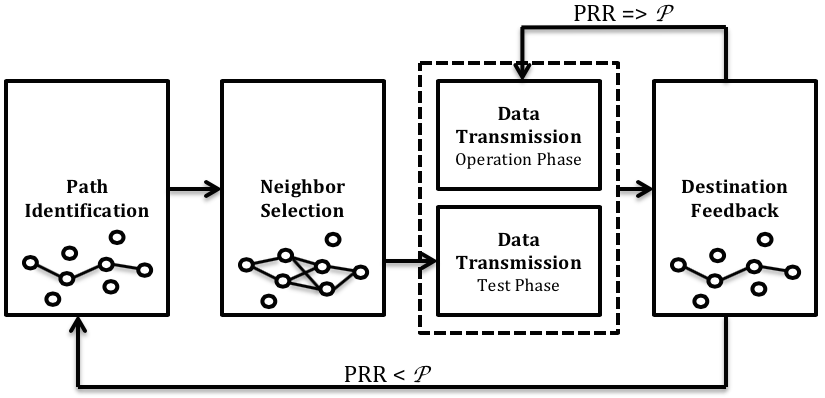
\includegraphics[height=4.5cm]{overview2.png}
\caption{Abstract structure of RFT Path Identification (see Section \ref{pathidentify}), Neighbour selection (see Section \ref{neighbourselection}).}
\label{fig:Overview}
\end{figure}

Path Identification module adopts two ways to identify the single paths that one node in each hop between the source and the destination. The first one employs the link quality control that any node forwards the the path identification packet only if received RSSI over the threshold. The adaptive tx power control is used in the second one. Any node adapts its tx power to the received signal strength. Low received signal is corresponding to low tx power and vice versa. Through these ways only qualified nodes would forward the path identification packet or transmit in the highest power. Thus capture effect enable the destination sequentially find two reliable paths. The destination prefers the first path, because the first path mandatorily restricts the minimum link quality. Should the too high threshold cause first way failure the destination uses the second path as backup.

Neighbour Selection module next selects neighbours for each relay node as helper nodes. Helpers in this paper are the one-hop neighbours of the relay nodes which are able to simultaneously receive and forward packets with relay nodes. The concurrent transmissions enhance the link quality and improve the reliability by constructive interference. RFT finds a number of helper nodes for the specific hops to reinforce the links, corresponding to the link quality of every hop in the identified path. In the end all the relay nodes and helper node are account for the data transmission between the source and the destination.

Data transmission module has two phases the test and the operation phase. New paths should be tested and if reliable then could be used in the operation phase. Normally the duration of the operation phase is much longer than the test phase. In the operation phase, the source sends a series of data packets to the receiver over a long time. If the PRR is below a certain threshold then RFT triggers the path identification phase again to find alternative paths. However, if the threshold is satisfied then RFT keeps using the paths for another operation phase. The threshold as the PRR metric ensure the reliability of the paths. 

In Destination Feedback module, the destination assesses the quality of currently used paths and decide if trigger the path identification module or not. All nodes open the radio at the moment and the destination floods the decision to the network. If no path update is needed irrelative nodes keep sleeping otherwise open radio for the following path identification. By this way much control overhead brought from Path Identification and Neighbour Selection modules can be saved.
%After finding new paths RFT firstly test the paths and if reliable then RFT will work in the operation phase. Normally the duration of the operation phase stay much longer than the test phase. If the PRR of the data transmission module (test or operation phases) is over the satisfactory threshold $\mathcal{P}$ (90\% in our implementation), the Destination Feedback module would not find new paths and directly jump to the operation phase of the data transmission module. If PRR is unsatisfied, the source will identify new paths and then launch the test phase. By this way the Destination Feedback module will update the paths only if necessary to against the radio environment variation. Therefore the PRR metric would be met given the predefined $\mathcal{P}$. Moreover this method saves much control overhead brought from Path Identification and Neighbour Selection modules.

Since constructive interference provides the network extremely tight time synchronisation, RFT employs static TDMA mechanism that all the time slots are equal. In the Data transmission module the majority of nodes will close the radio to save energy. Similar to LWB \cite{ferrari2012low}, RFT requires a node in the network to flood a synchronisation packet every second. Because of the TDMA mechanism RFT can easily be extended to support multiple source-destination pairs. If so one node need behave as the scheduler and adopt the schedule layer reported in LWB \cite{ferrari2012low}. Multiple sources then could sequentially run Path Identification and Neighbour Selection modules and transmit data packets in different time slots.

%RFT employs static TDMA mechanism that all the time slots are equal. In this way the Destination module can deterministic control the data flow and meet the PRR requirement. So RFT needs the global network time synchronisation as the prerequisite to realise TDMA and utilise constructive interference and capture effect. In the Data transmission module the majority of nodes will close the radio to save energy. To maintain the global network synchronisation one authorised node should flood a packet in each second to synchronise the sleeping nodes. Because of the TDMA mechanism RFT can easily be extended to support multiple source-destination pairs. If so the authorised node will behave as the scheduler and adopt the schedule layer reported in LWB \cite{ferrari2012low}. Multiple sources then could sequentially run Path Identification and Neighbour Selection modules and transmit data packets in different time orders.

%The key point of the systems is the first two modules, Path identification and Neighbour Selection. Although they have to identify the reliable path and helpers along the paths, this two modules would just last one or two seconds even for the network that has 100 nodes. The data packets will only be transferred in data transmission module and if the application need forward packets when other modules are operating, RFT have to stored the packets. For the duration of the first two modules are short, the latency can be neglected. The systems can reactive to channel dynamics quickly if we shorten the operation phase duration and increase path identification frequency without introducing much overhead and latency. The impact of the duration of the test phase and operation phase is evaluated in the section \ref{evaluation}.
\section{RFT: Detailed Mechanisms} 
\label{RFTdetail}
In this section we give the details of the main modules. Section \ref{pathidentify} presents how Path Identification module finds the reliable paths. Then Neighbour Selection module in section \ref{neighbourselection} is designed to add helper nodes for some weak hops and make use of constructive interference to consolidate these links. Section \ref{theoreticalanalysis} analyses the potential roles of the added neighbours and shows two instances in experiments. We assume all nodes have their own specific node IDs.% and reserve two arrays memory to store the nodes ID and received RSSI for the path finding and neighbour selection.
%And we believe that this task could be divided into two steps. First step is to identify one reliable and relative shortest path. Then the second step is to send reinforcements for some weak hops and make usage of constructive interference to consolidate these links and raise the packet delivery rate potentially. In the following we will show how to find the paths firstly.
\subsection{Path Identification}
\label{pathidentify}
As outlined in Section \ref{relatedwork} Sparkle proposes a path finding method for the source and the destination connection, which is fast and easy but the identified paths may not be reliable unfortunately. We further improve the method into two new ones, First Path and Second Path. Then the destination computes the number of required neighbours of every hop for the next Neighbour Selection module. In the end the destination floods the identified path and required neighbours information to activate the relay nodes of the path.

\emph{Path Identification Protocol:}
\begin{enumerate}
 \item Activate all nodes in the network. The source broadcasts a path identification packet which has two arrays, node IDs and received RSSI. The source add its node ID into the node IDs array. %This packet contains the series of node ID.
 \item \textbf{First path}: Any node that receives the path-ident packet should log its RSSI. Only if the packet RSSI is higher than the threshold $H$, this node can relay the packet once, meanwhile add its own ID and received RSSI value in the corresponding arrays.
 \item \textbf{Second path}: The mechanism is similar with above. The difference is the condition of relaying the path-ident packet. Whatever the packet RSSI is any node will relay it once. But the tx power will change pertaining to the RSSI. For low RSSI nodes use low tx power and high RSSI then high tx power.
  \item The destination will receive the path-ident packet containing the series of node IDs and RSSI. Node IDs stand for the path and RSSIs represent the link quality of every hop in the path. The destination then chooses the first path if available otherwise the second one. Mapping the RSSIs to the number of required neighbours as helpers for each hop in the end.%\textbf{Required Helpers Computation}:
  \item \textbf{Path Activation}: The destination floods a packet including the chosen path and number of required helpers of each hop to the network. The nodes contained in the path will mark themselves as relays and find neighbours in the Neighbour Selection module. The other nodes are waiting to be selected by relays.
 \end{enumerate}

The path identification packets, embedded with the nodes IDs and RSSI are mutually \emph{different} while in these packets dissemination. According to Section \ref{background} only Capture effect happens during the path finding process. Any node receives the strongest packet from the previous hop and rebroadcast it to the next hop, thus the destination can receive a series of node IDs as the identified path. Take Fig.~\ref{fig:ExpPathIdent} as the example to explain. We conceptually separate the network into 3 layers and multiple nodes are placed in each layer. Source node $S$ can directly connect with $A C E$. And these 3 nodes simultaneously broadcast their own path-ident packets. The destination $D$ can identify $E$ as a relay node, for $E$ has the strongest signal. This path $SED$ is the shortest but unfortunately very unstable. Two aspects cause the result. Capture effect help find the strongest link $ed$ but still too weak. $se$ is also fragile but this occasional connection gives $E$ opportunities to compete with $AC$ as the relay node. Thus the link quality control is needed to eliminate the fragile links. First Path and Second Path are proposed to tackle this issue.

In First Path all the nodes can relay the path-ident packet once only if they meet the received RSSI threshold $H$. In Fig.~\ref{fig:ExpPathIdent} $E$ could not meet $H$. That means $se$ is so weak that $E$ will not broadcast its ID and only $AC$ compete as the relay. In Second Path all nodes can relay the finding path packet but should adaptively change the tx power. In this case $E$ should lower its tx power because of the weak front link $se$. Then $ed$ would be too weak to reach $D$. The key idea behind First Path and Second Path is common that eliminating the fragile links. So through these two methods $AC$ concurrently broadcast their packets and $D$ cannot receive packets from $E$ anymore and keep waiting the incoming signal. $B$ only receive $A$'s and finally reach $D$. At last the destination $D$ finds $SABD$ as the path.

%If the identified paths come from this process, the signal loss of every link would be the smallest, and theoretically which means the paths would have the shortest hop counts from the source to the destination. This finding path method of Sparkle is effective but unreliable. It can ensure the identified node has good link quality with the next hop but cannot make sure the quality with the last hop. For instance, Fig.~\ref{fig:ExpPathIdent} shows the destination $D$ may find $C$ as relay but actually $C$ has bad connections with $S$. 
\begin{figure}
\centering
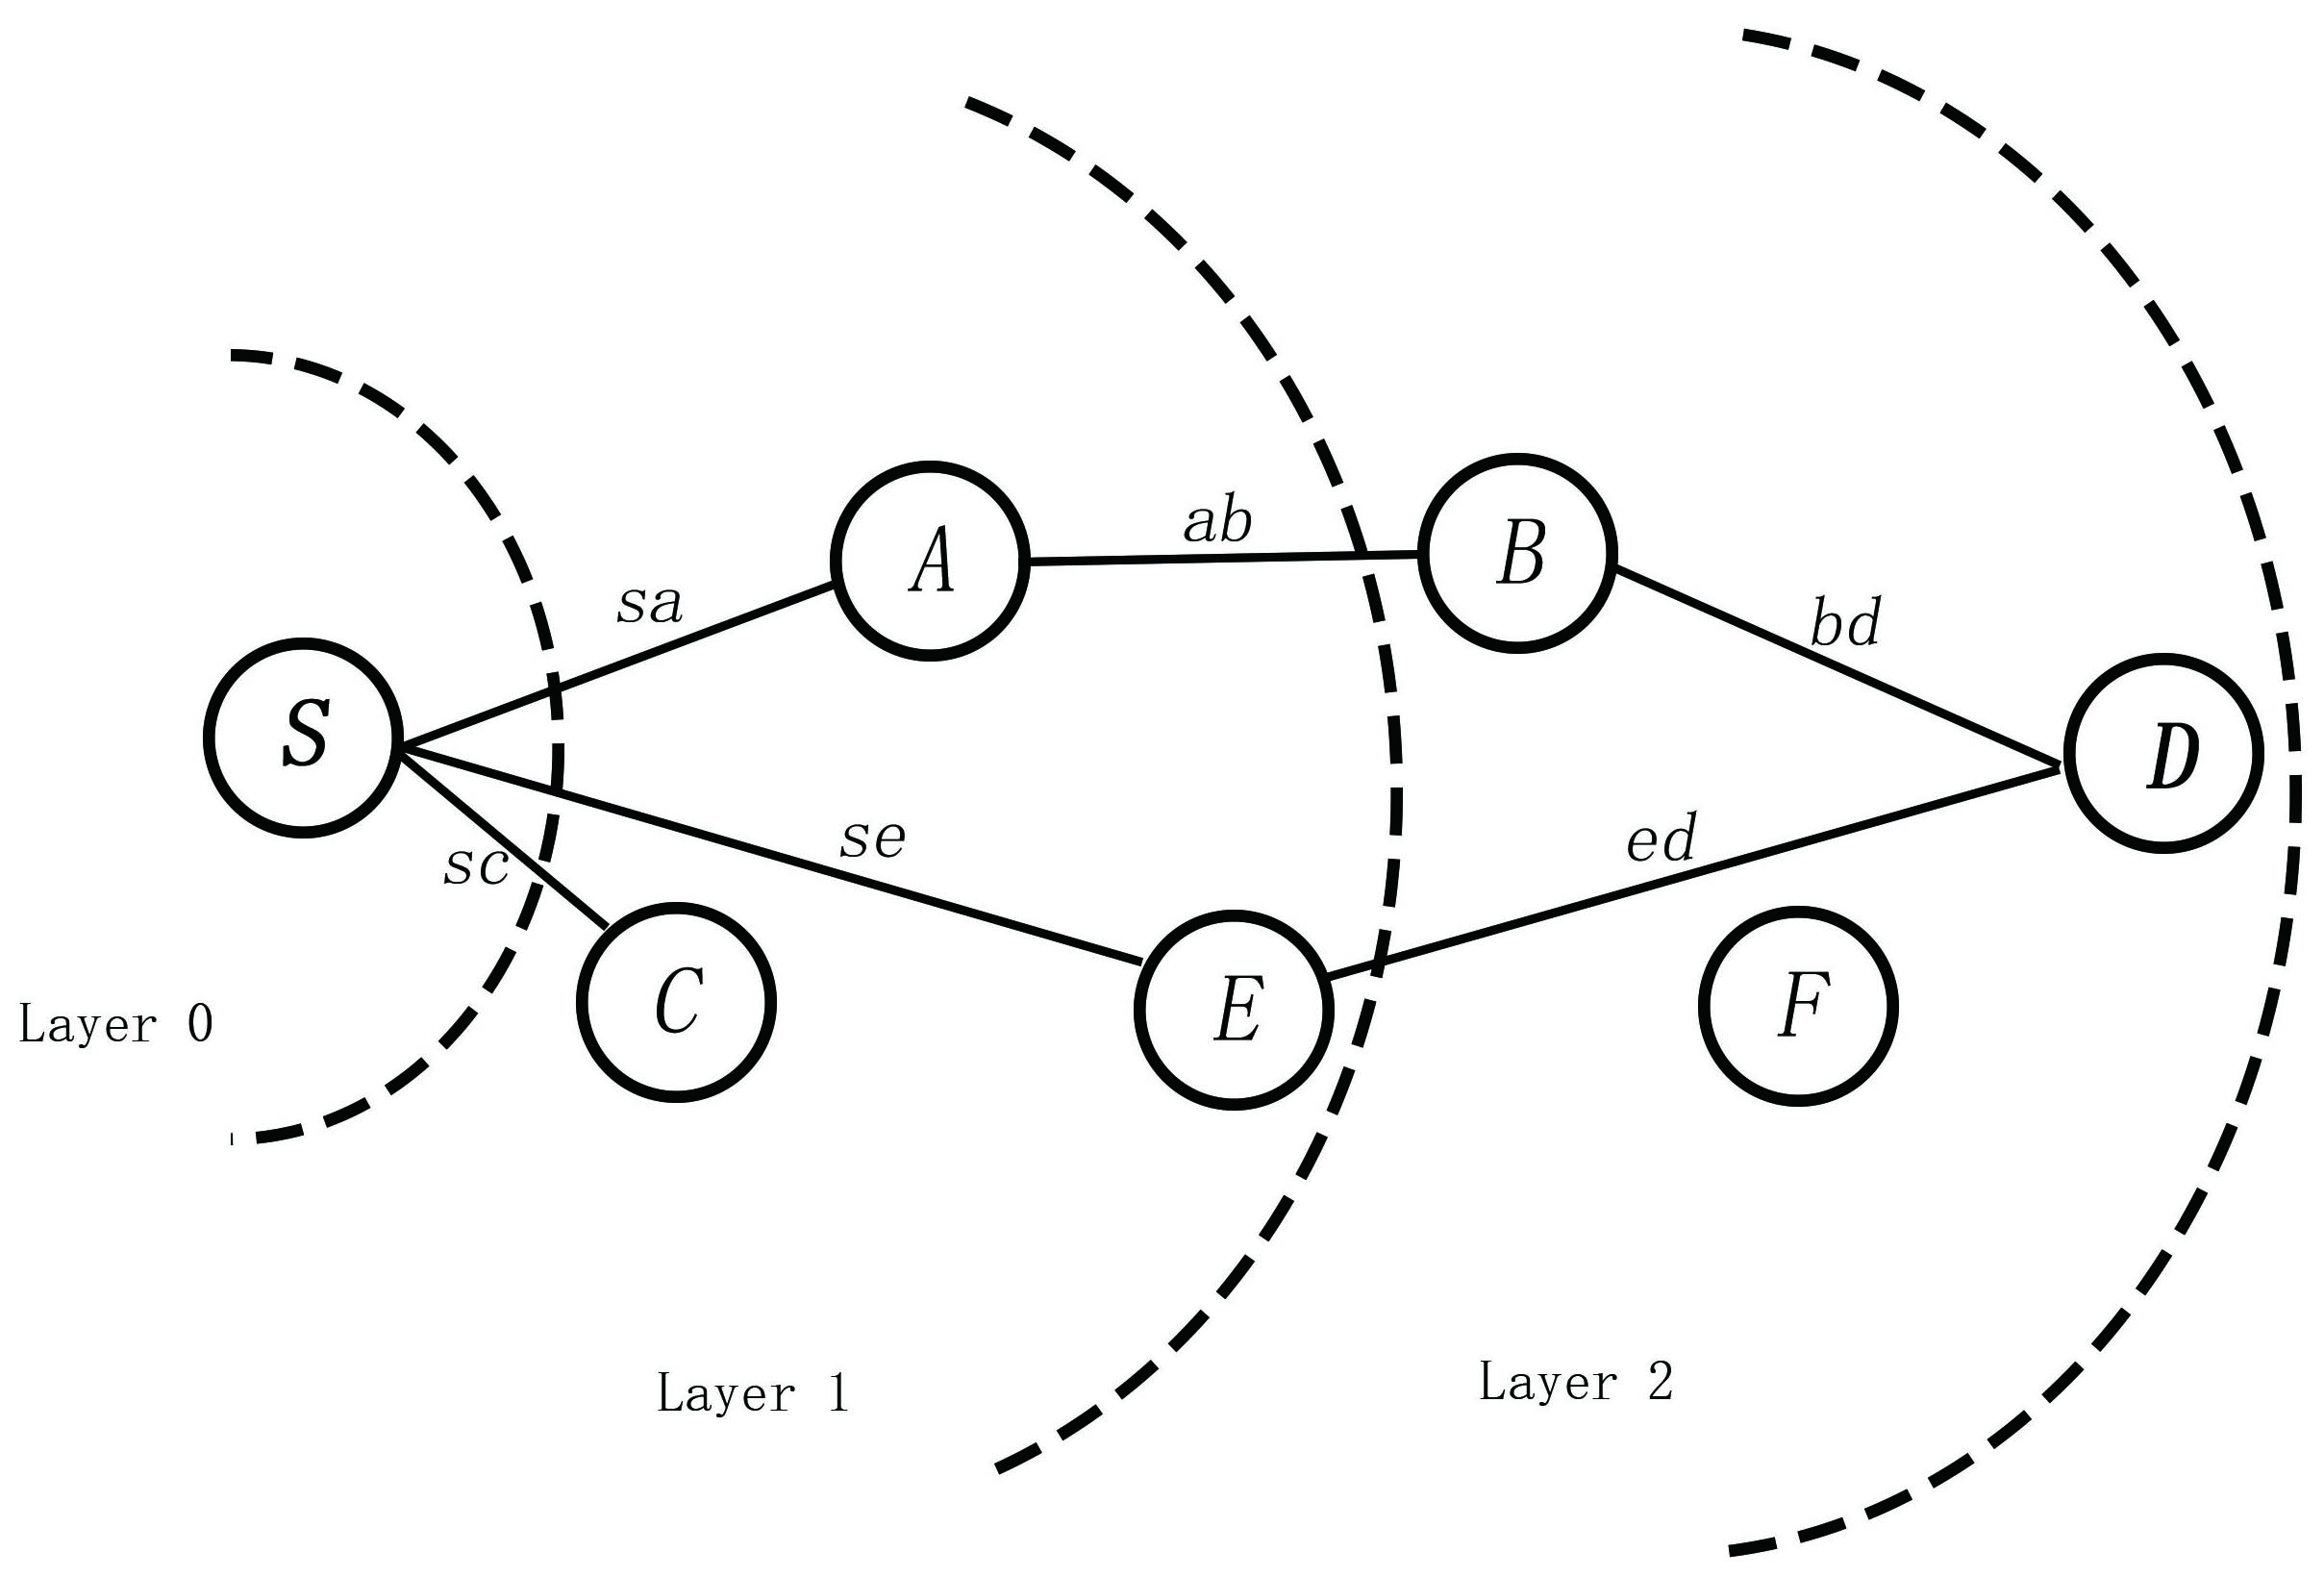
\includegraphics[width=7cm]{ExpPathIdent.jpg}
\caption{Example of Path Identification.}
\label{fig:ExpPathIdent}
\end{figure}

%On the contrary, the RSSI threshold of the First Path can ensure the quality of every link is over the threshold $H$. The Second path changes the transmit power of nodes according to the received signal strength. It lowers the probabilities that the bad nodes could be identified. Take node $B$ as example, $B$ has better connection with the source than $C$ and also has the good enough connection with $D$. Thus the higher transmit power of $B$ could help the destination $D$ find a better choice. %The reason is some nodes occasionally receive packets from the last node and they would have high chance to be selected as relays by next node, for they may have smaller signal losses or shorter distance with destination, etc.. However the link quality of first hop is weak and breakable. 

%Suppose there are three nodes $A, B, C$ between $S$ and $D$ and all three nodes occasionally and successfully receive the packet from $S$. $D$ would have high chance to receive packet from $C$ and the identified path should be $S, C, D$ but the link $SC$ could be very fragile. The end-to-end reliability of this path will be very low in this case. Thus we introduce the first path. The nodes will not relay packets unless its RSS is over the threshold $H$. For the second the nodes will lower the transmission power if its received RSS is low and higher the power if RSS is high.

Theoretically speaking First Path should be more reliable than Second Path. First Path mandatorily selects the qualified links over threshold $H$. The high $H$ undoubtedly ensure the high reliability. But it may require too many relays that bring the extra energy wastage. Also there may not exist the qualified links due to the unevenly network deployment. In our implementation we use the radio sensitive level as $H$ and Section \ref{sec:evaluationsetup} gives more details. Second Path gives the opportunities for those isolated nodes that only have weak connections with neighbours. In real experiments we find First Path is always available in most source-destination pairs. But for the specific pairs in the chaotic radio environment Second Path will be useful.

In the end the destination maps the array of received RSSI into the array of the number of required neighbours as helper nodes. The identified path surely still has unreliable links in some hops. The reliable link of the hop with high RSSI value need just few helper nodes and low RSSI need more helpers. Ideally multiple nodes in one hop can further increase the link quality by constructive interference. Neighbour Selection module selects the amount of helpers along the path to reinforce these links in the next. The mapping from the RSSI array to the Helper array is correlated to the hardware. Thus Section \ref{sec:evaluationsetup} shows the details. %Each relay node will identify the neighbours and concurrently forward data packets with them to strengthen the signal and improve the reliability.  The high RSSI of the hop require few helpers and vice versa. The array that containing the number of helpers needed in each hop will be used in Neighbour Selection module. 

%\subsubsection{How should we define the threshold $H$.}
%
%One of the important principles of path identification is to find the path that has few hop counts to the destination. If $H$ is too high, then the identified path certainly includes many redundant nodes and meaninglessly waste energy. Thus we define the sensitive level of radio chip as $H$ to provide us an relative reliable and shortest path. Since under the sensitive level, \cite{srinivasan2006and} and \cite{wu2008realistic} shows the radio chip would has the random packet reception rate from $0\%$ to $80\%$. Such kind of links are susceptible to noise, which is unreliable and unbearable. In our implementation, we use Tmote Sky and choose $-90 dBm$ as $H$, according to the datasheet. 
%\subsubsection{Mapping the RSSI to needed number of helpers.}
%Even we establish the signal threshold $H$ and automatically control the transmission power, the identified paths still may have fragile links. \cite{srinivasan2006and} and \cite{wu2008realistic} have done many experiments and show the similar the mapping from PRR to RSSI. The results show the PRR of RSSI value between $-75dBm$ to $-90dBm$ would be from $100\%$ to $85\%$ ideally. So we propose the Neighbour Selection module to further repair the lossy link and give the reinforcements to them. The computation of the number of the needed helpers is used for the following neighbour selection module. We establish the mapping from the RSSI value to the number of needed helpers. Our setting is the link over $-75 dBm$ do not need helpers, $-76dBm \sim -82 dBm$ need 1, $-83dBm\sim-90dBm$ need 2, and less than $-90dBm$ need 4 neighbours. In real experiment, the relays of identified path normally need 1 or 2 helpers. These setting could be changed by the different hardware. But we argue that the reasoning is universal and could be applied in other radio chips.

\subsection{Neighbour Selection} 
\label{neighbourselection}
After Path Identification module relay nodes know what the number of helpers are needed, how to efficiently select the appropriate neighbours would be an intractable problem. The relay node and the helpers for this relay should ideally have the same reliable links with nodes in the previous and next hop. Then all relays and helpers receive and forward packets simultaneously. To enable find such helpers, all one-hop neighbours of relays should setup the neighbour table to know if they have good connections with relays. Instead of traditional unicast which costs excessive control overhead and latency, RFT protocol locally establishes the neighbour table and distributively find the additional neighbours.

\emph{Neighbour Selection Protocol:}

Capture effect dominates this protocol and efficiently help nodes to identify neighbours as concurrent transmitters. Since nodes may have more than 10 to 20 neighbours in the dense deployment cases like the testbed \cite{doddavenkatappa2012indriya} we used, one node has no chance to decode a packet if all its neighbours simultaneously broadcast different packets in the same transmission power. The highest signal will not be 3dB higher than the sum of the others. To meet this challenge, through 3 following steps we establish the neighbour table and perform the dynamic power control technique to identify neighbours and activate these nodes at last. Fig.~\ref{fig:NeighborSelection} shows the details of the protocols.

Neighbour Selection process has three main procedures. The first step is the neighbour table establishment. All relays sequentially broadcast a packet to one-hop neighbours to acknowledge the connections. Should received this acknowledge packet neighbours insert this relay as an entry into the table and log the received RSSI value. In previous path finding module the neighbours of the source and the destination have already logged the connections and RSSI values. In the end all one-hop neighbours of the identified path have established the neighbour table and RSSI table. The state of connections with relays is used for the computation of tx power levels.

%  by the connections and link qualities of the neighbour table. The logic behind is: the more helpful neighbours transmit in higher power; the less helpful ones transmit in lower power and the others do not give feedback. 
\begin{figure*}[!t]
\begin{minipage}[!t]{0.73\linewidth} 
\centering
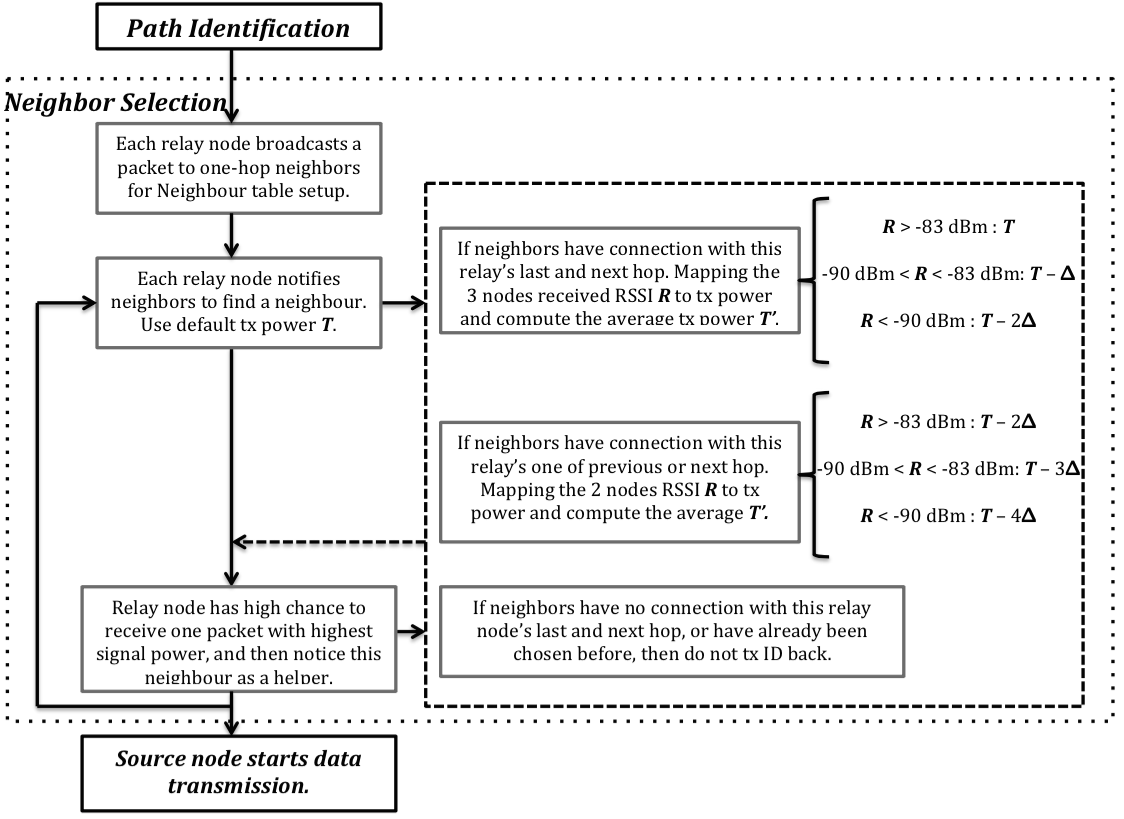
\includegraphics[height=9.5cm]{NeighborSelectionPctl2.png}
\caption{Neighbour Selection process. Neighbours change the tx power based on neighbour table and RSSI table. In our implementation default $\Delta$ is 5 dBm.}
\label{fig:NeighborSelection}
%\end{figure*}
\end{minipage}
\hfill
\begin{minipage}[!t]{0.25\linewidth} 
%\begin{figure}
\centering
\subfigure[Neighbour table setup]{
\begin{minipage}[b]{0.8\textwidth}
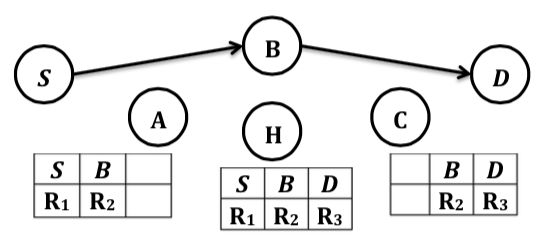
\includegraphics[width=3.7cm]{Exp_ns_step1_3.png}
\end{minipage}
}
\subfigure[Relay Node requests Helpers]{
\begin{minipage}[b]{0.8\textwidth}
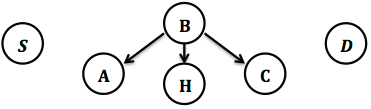
\includegraphics[width=3.7cm]{Exp_ns_step2.png}
\end{minipage}
}
\subfigure[Neighbours send Feedback]{
\begin{minipage}[b]{0.8\textwidth}
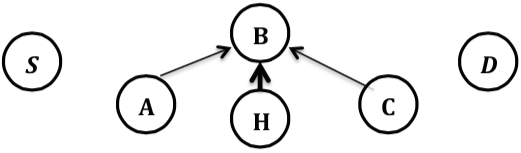
\includegraphics[width=3.7cm]{Exp_ns_step3_2.png}
\end{minipage}
}
\subfigure[Relay receive message from neighbours and notify H as Helper]{
\begin{minipage}[b]{0.8\textwidth}
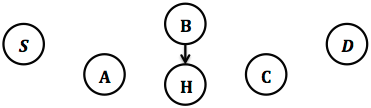
\includegraphics[width=3.7cm]{Exp_ns_step4.png}
\end{minipage}
}
\subfigure[Multiple nodes in the same hop strengthen the link quality]{
\begin{minipage}[b]{0.8\textwidth}
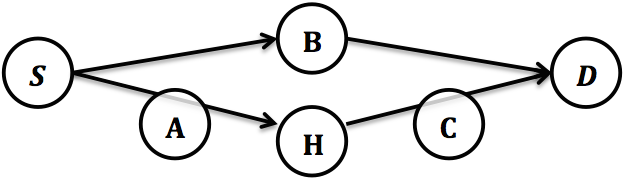
\includegraphics[width=3.7cm]{Exp_ns_step5.png}
\end{minipage}
}
%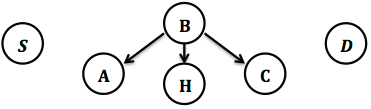
\includegraphics[width=3cm]{Exp_ns_step2.png}
%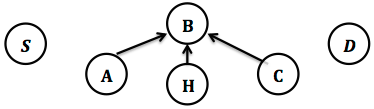
\includegraphics[width=3cm]{Exp_ns_step3.png}
%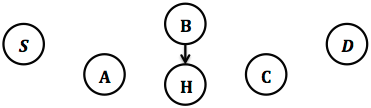
\includegraphics[width=3cm]{Exp_ns_step4.png}
%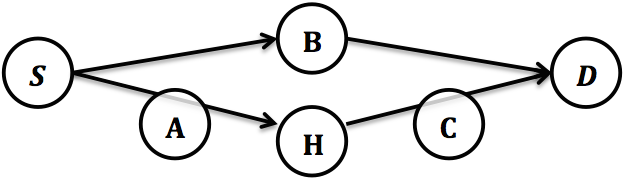
\includegraphics[width=3cm]{Exp_ns_step5.png}
\caption{Example of the Neighbour Selection process.}
\label{fig:ExpNeighborSelection}
\end{minipage} 
\end{figure*}

The next step is the neighbour selection process. One relay node broadcasts a notification packet to request one helper node. Every one-hop neighbour then sends back its ID in the modified tx power at the same time. The tx power control significantly reduce the number of concurrent transmissions and the relay node has high chances to detect the helper node. The mapping of the tx power is based on the theory that the neighbours with reliable connections with relays transmit in higher power; the others transmit in lower power or close the radio. The ideal helpers should qualifiedly link with 3 nodes, the local and two adjacent relays in the previous and next hop. Only these neighbours can be the qualified concurrent transmitters for the relay nodes and strengthen the signal by Constructive interference. %These ideal helpers will have the highest tx power.

Specifically neighbours transform the RSSI of each Neighbour table entry to transmission power levels. For the low RSSI the default tx power $\mathbf{T}$ are subtracted from $\Delta$s. Two or three entries, the local and the adjacent relays, will be mapped and averaged to $\mathbf{T'}$ as the modified tx power. Neighbours then concurrently transmit their IDs in different $\mathbf{T'}$ to the relay and therefore the relay will identify the helper by capture effect. The details of neighbour selection process has been illustrated in Fig.~\ref{fig:NeighborSelection}. The path identification process enable find one helper for each time and relay nodes will loop the process multiple times to find a number of helpers according to the Path Identification module. The final step is the helper activation. The specific neighbours are informed and activated in the following data transmission period. Fig.~\ref{fig:ExpNeighborSelection} shows a typical procedure that how the relay node $B$ identifies the helper $H$ which owns reliable links with $S B D$.



%Neighbours decrease the default tx power $\mathbf{T}$ by $\Delta$s based on the RSSI table for each Neighbour table entry, see Fig.~\ref{fig:NeighborSelection}. Two or three entries, the local and the adjacent relays, will be mapped and averaged to $\mathbf{T'}$ as the modified tx power. The ideal neighbours as helpers which own qualified links with 3 nodes, the local and two adjacent relays in the previous and next hop, will have the highest tx power. Only these neighbours can be the qualified concurrent transmitters for the relay nodes and strengthen the signal by Constructive interference. Neighbours then concurrently transmit their IDs in different $\mathbf{T'}$ to the relay and therefore the relay will identify as the helper node by capture effect.

%The mapping of the tx power is based on the theory that the neighbours with reliable connections with relays transmit in higher power; the others transmit in lower power or close the radio. The details of neighbour selection process has been illustrated in Fig.~\ref{fig:NeighborSelection}. The path identification process enable find one helper and each relay will loop the process multiple times to find a number of helpers according to the Path Identification module. The final step is the helper activation. The specific neighbours are informed and activated as the helpers in the following data transmission period. Fig.~\ref{fig:ExpNeighborSelection} shows a typical procedure that how the relay node $B$ identifies the helper $H$ which owns reliable links with $S B D$.

All three steps are very fast and only need few transmission slots. One time slot $t$ contains one reception and one transmission. In our implementation, the duration of one slot is 0.1 second. Suppose 3 relays are between the source and the destination and each relay needs 1 helper. Each relay needs 1 $t_1$ slot for neighbour table setup. One helper costs 2 $t_2$ slots to be selected as mentioned above. Synchronisation in per second need 1 $t_{syn}$. If we consider the path identification, it needs 2 $t_0$ slots. In all, the source only needs $12t$ which is 1.2 seconds to build up the link and then start data transmission.
\begin{equation}
\begin{aligned}
&t_0 = t_1 = t_2 = t_{syn} = t \\
%\end{equation}
%\begin{equation}
&\mathcal{T}_p = 2 * t_0 \\
%\end{equation}
%\begin{equation}
&\mathcal{T}_n = 3 * t_1 + 3 * 2 * t_2 \\
%\end{equation}
%\begin{equation}
&\mathcal{T}_{all} = \mathcal{T}_n + \mathcal{T}_p + t_{syn} = 12 t
\end{aligned}
\end{equation}

It is worthy to mention that we consider these kind of neighbours which only connect with two relays, like $A$ or $C$ in Fig.~\ref{fig:ExpNeighborSelection}. We suppress the tx power of this kind of nodes, nevertheless they are beneficial as cooperators in some situations where no ideal helpers exist, especially around the source and the destination.  Although it may bring the additional energy cost, we still give the opportunities for these nodes to increase reliability. All these settings in the Fig.~\ref{fig:NeighborSelection} are based on TelosB motes and the theory could be applied to any other hardware. 

\subsection{Benefits of Helpers}
\label{theoreticalanalysis}
This section studies RFT analytically. In particular, we are especially focused on the benefits to the end-to-end reliability brought from the helper nodes.

We consider the network structure in Fig.~\ref{fig:theoreticalanalysis}. It simplifies the multiple hops and transmitters network. Node $R$ stands for one identified relay and $H$ is on behalf of one helper. In this way, we reconstruct all the potential scenarios in the sense that all the possible roles the helper could behave in terms of concurrent transmitters or cooperators. 

%We first present the probability analysis of four situations and then apply the conclusions into the implementation of the RFT protocol. The results show that the mechanism of the appropriate helpers could make use of constructive interference and increase the end-to-end reliability.
\begin{figure}[!t]
\centering
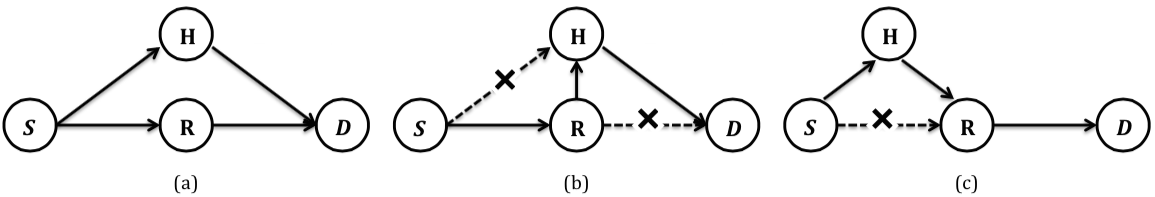
\includegraphics[width=9cm]{theoreticalanalysis_cut.png}
\caption{Three potential situations the helpers may face. (a) is the ideal situation that the helper has good connection with the other three nodes. (b) (c) the helper acts as an cooperator.}
\label{fig:theoreticalanalysis}
\end{figure}

When relays select the potential neighbours to help forward data packets, these neighbours may have three potential situations. The most ideal situation Fig.~\ref{fig:theoreticalanalysis}$(a)$ is both of the helper and the relay could receive the packets from $S$ and route these packets to $D$. The link of the second hop is entirely depends on the constructive interference. (b) is the helper or the relay cannot forward to $D$ but still has the second chance to pass packets aside and try again. (c) is the helper can only setup connections with two out of three nodes. The last two cases will increase 1 hop count, which can be illustrated in the experiment results if these cases happen. 

\begin{figure*}[!t]
\centering
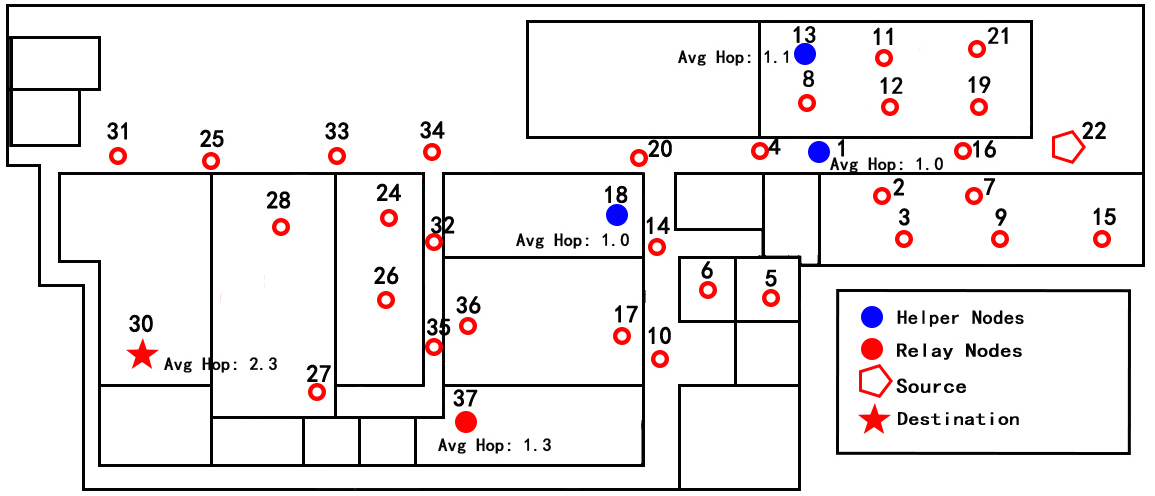
\includegraphics[height=7cm]{withLinkQuality3.jpg}
\caption{Average hop count distance of the helpers and relays in one instance.}
\label{fig:hopcountexample}
\end{figure*}

%\begin{table}[!t]
%\renewcommand{\arraystretch}{1.3}
%\caption{An Example of Average hop count distance of the helpers and relays}
%\label{table_example}
%\centering
%\begin{tabular}{|c|c|c|c|}
%\hline
%Helper No. & Hop Count & Relay No. & Hop Count \\ \hline
%10     & 1         & 6     & 1.1       \\ \hline
%59     & 3         & 33    & 2         \\ \hline
%40     & 3.8       & 55    & 3         \\ \hline
%66     & 4.7       & 44    & 3.8       \\ \hline
%116    & 5.9       & 64    & 4.3       \\ \hline
%123    & 6.3       & 129   & 5.3       \\ \hline
%       &           & 135   & 6.3       \\ \hline
%\end{tabular}
%\end{table}

Fig.~\ref{fig:hopcountexample} shows the average hop count distances of the identified helpers and relays in two experiments. The helpers mostly locate the same distance with the relays which means they concurrently transmit packets and exploit the constructive interference to improve the end-to-end reliability. Since we impose the restrictions on the link qualities when finding the path at first, the relays and helpers can always receive packets simultaneously, like the ideal case $(a)$ in Fig.~\ref{fig:theoreticalanalysis}. The helpers in some hops have shorter distance than the relays. It indicates that the case $(c)$ may happen in low possibilities. We argue that although constructive interference is able to strengthen the signal power, but the prerequisite is multiple transmitters should receive packets at the same time. Thus it is better not select the nodes with extremely low RSSI values and their neighbours would not bring much benefits. 

%\paragraph{Mapping the RSSI to needed number of helpers.}
%The implementation of RFT protocol is on Tmote Sky devices. According to several papers like \cite{srinivasan2006and} and  \cite{wu2008realistic} , the PRR curve corresponding to the RSSI value remains at the ideal level and then drop deeply into zero reception rate at $-90\sim-93dBm$. The variation area of PRR has two specific phases. In $-76\sim-82dBm$ section, the PRR would slowly drop from 100\% to 85\% or 80\%. And in the $-83\sim-90dBm$ block PRR could drop down to 20\%. Below $-90dBm$ PRR tempts to have random reception rate even dropping to zero. If the source chooses relays with $-91$ below $-90dBm$, $p_{SR}$ and $p_{SH}$ could be very low and $\mathbb{P}_{S \to D}$ is same as well. Thus based on the analysis above we define the lower bound $-90dBm$ for the First Path in the path identification protocol, in order to eliminate the negative packet reception rate fluctuation. And recent papers like Chaos\cite{landsiedel2013chaos} and Splash\cite{doddavenkatappa2013splash}, and the experiments in our lab have shown that more than three concurrent transmitters may cause the destructive interference and lower the reliability. Thus we set the needed number of potential helpers for $-76 \sim -82dBm$ section is one, $-83\sim-90dBm$ is two, and below $-90dBm$ is four. Through this mapping the selected helpers could have high chance to behave in the ideal case like in Fig.~\ref{fig:theoreticalanalysis} (a).

\section{Evaluation}
\label{evaluation}
In this section we evaluate the performance of RFT through extensive testbed experiments. The impact of Neighbour Selection upon the delivery rate and the comparison with Sparkle in terms of energy efficiency and reliability have been investigated. We use the testbed Indriya \cite{doddavenkatappa2012indriya} to evaluate all the features and performances of protocols. The testbed deploys TelosB nodes in university buildings. The presence of students and co-located Wi-Fi have created the realistic experiment environment. During our experiments period Indriya has 100 nodes available to use. 
 
\emph{Metrics:}
We consider four key performance metrics: (a) Latency is the time between the source node transmits data packets and the destination node receives; (b) Energy consumption is evaluated in Joule in terms of the control overhead and data transmission; (c) Packet Reception Rate (PRR) is the percentage of packets received at the destination; and (d) radio duty cycle is the average fraction of time a node has the radio turned on for all the packets delivery. We compute the energy consumption based on radio-on time of nodes, and measure the radio-on time in software using Contiki's power profiler.
\subsection{Evaluation Setup.}
\label{sec:evaluationsetup}
RFT is implemented in Contiki OS \cite{dunkels2006contiki} on Tmote Sky platform. The design is based on Chaos protocol, but the other functions except data processing have all been eliminated. And the default configuration of the processing time, MCU clock cycles, is 1700. This corresponds to a processing time of $0.4$ms as the definition of MCU clock frequency in Chaos. This time is sufficient for the neighbour table setup and transmission power reactive changes. The other tasks like the paths selection and the computation of required helpers is executed after turing off radio, called post-processing. Since Chaos would not turn off the radio during the data processing time, only the real-time tasks is scheduled between the transmission and reception slots and the others are moved to the post-processing period.

We also implement Sparkle in the testbed. The default of the test phase as 100 seconds and data dissemination phase as 1000 seconds, which is fair to compare two protocols. To make the diameter of the network extend to multiple hops, the default transmission power of TelosB node is -3 dBm without the specific declaration. Each experiment lasts over half hour and we repeat experiments over 5 times to evaluate each protocol in the different time zone, like morning, afternoon or midnight. Both protocols transmit 10 packets in every second and data transmission rate is 9 packets per second. But for Sparkle the path identification slot if needed can lower the data transmission rate to 8 packets per second.

\paragraph{How should we define the threshold $H$}
One of the important principles of path identification is to find the path with few hops. If $H$ is too high, then the identified path certainly includes many redundant nodes and meaninglessly waste energy. Thus we define the sensitive level of radio chip as $H$ which contributes to an relative reliable and shortest path. Since under the sensitive level, \cite{srinivasan2006and} and \cite{wu2008realistic} shows the radio chip would has the random packet reception rate from $0\%$ to $80\%$. Such kind of links are unreliable and susceptible to the noise. The implementation of RFT protocol is on Tmote Sky devices, therefore according to the datasheet we choose $-90 dBm$ as $H$ to eliminate the negative packet reception rate fluctuation. 
\paragraph{Mapping RSSI to requried number of helpers}
According to papers \cite{srinivasan2006and} and  \cite{wu2008realistic} , the PRR curve versus RSSI value remains at the ideal level and then drop deeply into zero reception rate at $-90\sim-93dBm$. The variation area of PRR has two specific phases. In $-76\sim-82dBm$ section, the PRR would slowly drop from 100\% to 85\% or 80\%. And in the $-83\sim-90dBm$ block PRR could drop down to 20\%. Thus we set the needed number of potential helpers for $-76 \sim -82dBm$ section is one, $-83\sim-90dBm$ is two, and below $-90dBm$ is four. Through this mapping the selected helpers could have high chance to behave in the ideal case like in Fig.~\ref{fig:theoreticalanalysis} (a) and insure the high reliability.
%If the source chooses relays with $-91$ below $-90dBm$, $p_{SR}$ and $p_{SH}$ could be very low and $\mathbb{P}_{S \to D}$ is same as well. 

\subsection{Benefits of controlled path identification and helpers.}
\label{sec:benefitsofhelpers}
We evaluate the impact of the controlled path identification and neighbour selection modules. We let the source identifies one single path without RSSI threshold and power control, short as Single Path protocol. The path identification mechanism of Sparkle can be seen as the combination of multiple Single Paths. We compare Single Path and Sparkle with RFT to evaluate the benefits of the controlled path identification and additional helpers. 

Two traffic flows have been executed. The first flow has short hops, both the source and destination are in the third floor of the testbed. The average hop count is 3 in the default transmission power. The other traffic flow has the same source but the destination locates in the first floor which almost over 5 hops away from the third floor. Our each experiment runs 30 minutes and repeat more than five tests in different time of the day. More than ten thousand data packets are transferred in each test. 
\begin{figure}
\centering
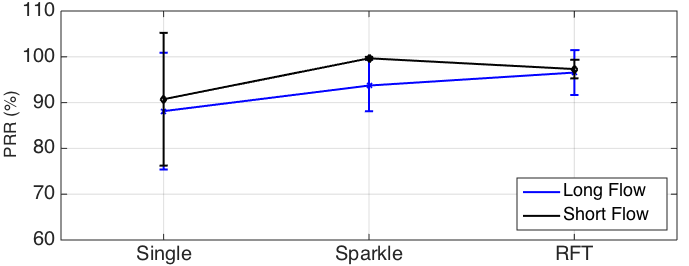
\includegraphics[height=3.55cm]{errorbar_prr_single_sp_rft.png}
\caption{The comparison of the end-to-end packet reception ratio of Single Path, Sparkle and RFT RFT is more robust than the other two modes.}
\label{fig:prr_error_single}
\end{figure}
%\paragraph{Finding 1:}

\emph{Finding 1:} 
RFT improves the average end-to-end PRR by about 10\% than the Single Path. RFT and Sparkle have almost same PRR but RFT is more robust.

Fig.~\ref{fig:prr_error_single} shows the mechanism, controlled path identification and neighbour selection has help RFT to be more robust than Single Path. The PRR of the Single Path has the severe variation and the minimum PRR could drop below 80\%. The Single Path may occasionally choose the nodes with fragile links that are easy to be interfered and therefore cannot reliably deliver packets in the data transmission module. While Sparkle has comparable PRR, RFT has lower variation and more robust than Sparkle.
\subsection{Impact of network diameter and packet size}
\label{sec:txpwr&pktsize}
Next we investigate the influence of the network diameter and packet size upon the performance of RFT. 
%\paragraph{Finding 2:}

\emph{Finding 2:} 
RFT efficiently supports different network diameters and packet size. RFT has the similar extremely low duty cycle with Single Path protocol but provide over 90\% satisfactory end-to-end reliability. 
\subsubsection{Scenarios}
To evaluate the network diameter, we vary the transmission power of TelosB nodes from -10 dBm to 0 dBm. The diameter of the network could be up to 7 hops. To test the influence of packet size, we vary the packet size from 42 to the maximum 128 bytes.
\begin{figure}
\centering
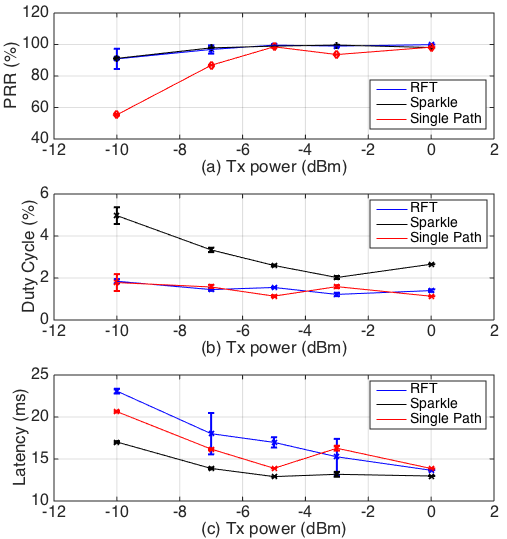
\includegraphics[width=9cm]{errorbar_defaultpower2.png}
\caption{Impact of transmit power. RFT provide the satisfactory reliability and extremely low duty cycle and latency. The packet size is 42 bytes in these series experiments.}
\label{fig:power}
\end{figure}
\subsubsection{Results}
Fig.~\ref{fig:power} shows RFT provides the satisfactory reliability that more than 90\% in all different transmit power settings. The linearly changes of PRR, duty cycle and latency with transit power is reasonable, since the lower tx power means the longer hop counts and less reliability of links. But the mechanisms of RFT can provide the satisfactory reliability as Sparkle shown in subfigure (a) and maintain extremely low duty cycles like Single Path, see subfigure (b). RFT brings few more milliseconds latency which used for the data processing before forwarding packets to the next hop, but the duty cycle of RFT could be 2.5 times lower than Sparkle.
\begin{figure}
\centering
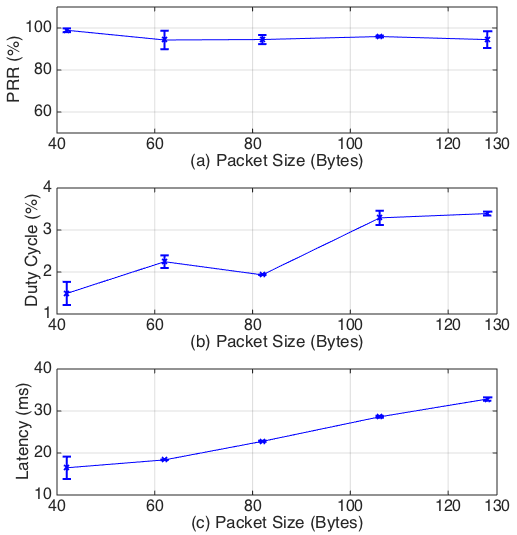
\includegraphics[width=9cm]{errorbar_payload_new2.png}
\caption{Impact of packet size. Large packet size does not affect the reliability and reasonably increase the duty cycle and latency, because of the increasing length of transmission and reception duration. The transmit power is -5 dBm.}
\label{fig:payload}
\end{figure}
We can learn from Fig.~\ref{fig:payload} that the large packet size has no noticeable influence upon the reliability. The average PRR is 97\%, even large packets are more susceptible to the channel fluctuation. The length of packets increase the duty cycle and latency, because the transmission and reception slot increase correspondingly. 

\subsection{Impact of the RSSI threshold in the First Path}
\label{sec:thrssi}
In this section we examine how the RSSI threshold $H$ affects the path identification and neighbour selection process and find which $H$ would be more appropriate in real scenarios.
%\paragraph{Finding 3:}

\emph{Finding 3:} 
The higher RSSI threshold $H$ incurs that the more relay nodes are identified in the path and less helpers are needed, and the lower $H$ causes less nodes as relays in the path and more nodes as helpers. The $H$ lower than $-90dBm$ may cause the network unsteady. The PRR of the destination could drop to around 90\%. But in all situations, $H$ does not have much influence upon the PRR and duty cycle of the network.
\subsubsection{Scenarios}
When the source node finds the First Path, the prerequisites that any node rebroadcasts the path identification packets and have the chances to be closed as relays, is their received RSSI is over the threshold $H$. The $H$ value compulsively limits the minimum signal strength of the identified links. The high $H$ strictly requires the qualified nodes as relays. Should such nodes exist in all locations too many nodes will be identified as relay nodes and cause additional energy consumption. We never consider the extremely high $H$ which may cause the path identification failure. In this section we investigate the $H$ value from $-98$ to $-76 dBm$ to see its impact upon the packet delivery.
\begin{figure}
\centering
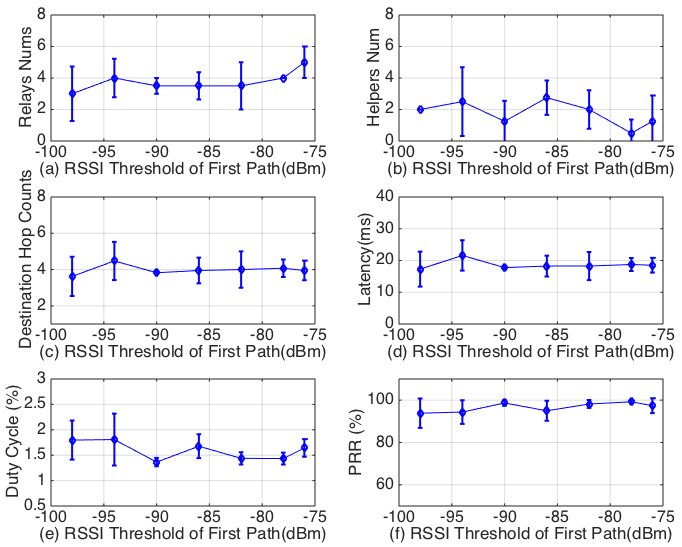
\includegraphics[height=7.4cm]{errorbar_thrssi_ANS3.png}
\caption{The impact of the RSSI threshold in the First Path.}
\label{fig:testthrssi}
\end{figure}
\subsubsection{Results}
We can learn from Fig.~\ref{fig:testthrssi} that RFT finds more nodes as relays associated with the $H$ growth trend. It is because the strict signal strength threshold requires the relays locate close to each other, which need more nodes than the undemanding threshold. Correspondingly Fig.~\ref{fig:testthrssi} (b) shows RFT finds fewer helper nodes for the identified path as $H$ rises. The reason clearly is the path with lots of relays has few weak links therefore less helper nodes are needed. Thus the higher $H$ requires more nodes as relays in the path but fewer as helpers, the lower $H$ demands fewer nodes as relays but more as helpers. But the low $H$ may affect the reliability of the identified path and result in the relatively unsteady PRR. Therefore $-90 dBm$ as the sensitive level of the radio chip is determined as the default signal strength threshold.


\subsection{Impact of the Delta}
\label{sec:testdelta}
In this section we examine how the RSSI delta settings in the Neighbour Selection module affect the effectiveness of identifying neighbours.
%\paragraph{Finding 4:}

\emph{Finding 4:} 
The relative large delta is beneficial to distinguish the neighbours and identify the helpers.
\subsubsection{Scenarios}
After the relay nodes setup the neighbour tables and received RSSI tables, they have to estimate the modified transmit power. Since the deployed network could be very dense, these neighbours should variate the power in order to let the relays identify one best neighbour by the capture effect. Thus the neighbours will discriminate the transmit power by the delta depending on the neighbour tables and the received RSSI tables, see the protocol in Fig.~\ref{fig:NeighborSelection}.
\begin{figure}
\centering
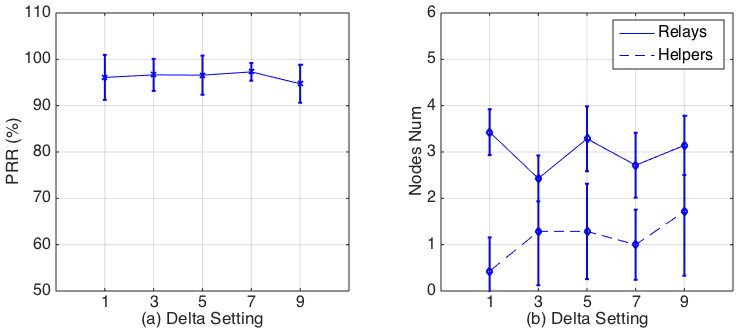
\includegraphics[height=3.87cm]{errorbar_delta3.png}
\caption{The impact of the Delta setting.}
\label{fig:testdelta}
\end{figure}
\subsubsection{Results}
From Fig.~\ref{fig:testdelta} we can see that the RFT has the higher probabilities to find helpers if the delta grows larger. We can see the higher delta contribute to more helpers. Actually the network density influence the effectiveness of finding neighbours behind and the variation of the delta value in adaptive ways could be the future work. For the testbed the default delta value is 5 which provides sound reliability.

\subsection{Impact of the number of required helpers}
\label{sec:numhelpers}
In this section we examine how the mapping from RSSI values to the number of required helpers affects the protocol performance.
%\paragraph{Finding 5:}

\emph{Finding 5:} 
The relative larger number of helpers setting contribute to more nodes been identified. More helpers been identified theoretically strengthen the network reliability but slightly increase the network duty cycle.
\subsubsection{Scenarios}
The nodes as relays in the identified path need find a number of neighbours as helpers according to the required helpers settings in different RSSI sections. In the default setting the $-76 \sim -82dBm$ section needs 1 helper and $-83\sim-90dBm$ needs 2 helpers. In this section we evaluate three other setting pairs, 0 and 1, 2 and 3, 3 and 4, which may gradually lead more nodes to be identified as helper nodes.
\begin{figure}
\centering
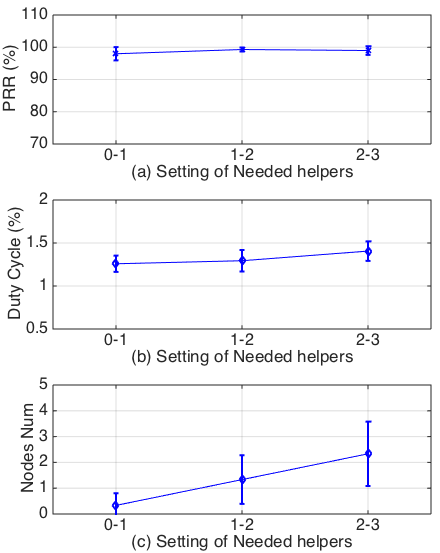
\includegraphics[width=7cm]{errorbar_numshelpers_ANS2.png}
\caption{The impact of the number of required helpers setting.}
\label{fig:testnumhelpers}
\end{figure}
\subsubsection{Results}
We can learn from Fig.~\ref{fig:testnumhelpers} that the PRR of RFT remains steady and the duty cycle increases slightly. Since the higher number of required helpers can lead to identify more neighbours as helper nodes, the network duty cycle reasonably rises 0.1\% or 0.2\%. On the other hand, the number of the identified helpers linearly increases as the network changes from the 0-1 pair to the 2-3 pair. Theoretically speaking the more helpers identified the more reliability the network may have and the duty cycle of the network does not remarkably increase. Thus the 1-2 and 2-3 setting pair would be recommended for the users in real applications. 

\subsection{Impact of test and operation phase duration}
\label{sec:testphase&operationphase}
In this section we investigate how the duration of the test and operation phase affect the RFT performance. 
%\paragraph{Finding 6:}

\emph{Finding 6:} 
The relative long test phase is beneficial to make RFT more reliable. RFT remains high energy efficiency even when the source find paths in high frequency.
\subsubsection{Scenarios}
We evaluate three settings, 10s test phase and 100s operation phase, 10s / 1000s and the default 100s / 1000s. The destination would shift the duration, test or operation phase, based on the PRR of the previous phase.
\begin{figure}
\centering
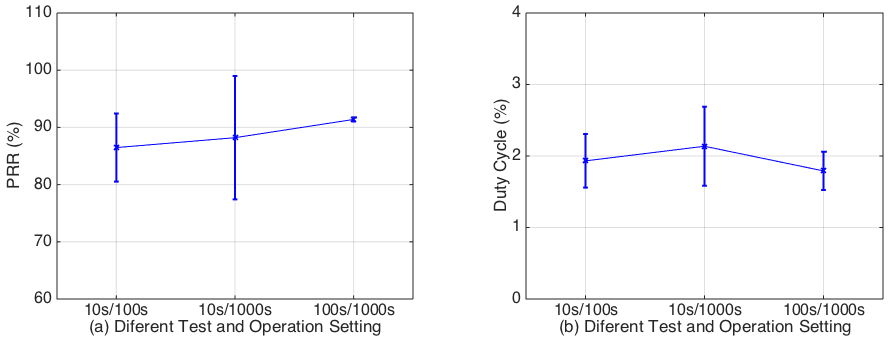
\includegraphics[height=3.55cm]{errorbar_testphase3.png}
\caption{The impact of test and operation phase duration.}
\label{fig:testphaseduration}
\end{figure}
\subsubsection{Results}
We can learn from Fig.~\ref{fig:testphaseduration} that the performance of RFT remains steady but a relative longer test phase is better.  Our the PRR satisfactory threshold is 90\% which is quite strict for 10s to differentiate if the link quality is good or not. We specially examine -10dBm, the low transmit power case, in which the channel fluctuation is severe. RFT may keep update paths to find one with 90\% PRR which affect the reliability and energy efficiency. Thus the relative long period of path testing is better. Duty cycle keeps extremely low and variate by only 1\% or 2\%. Thanks to the high energy efficiency of Path identification and Neighbour selection protocols, RFT remains high energy savings even the source finds path every 10s in the worst-case settings.  

\subsection{Comparing RFT}
\label{sec:ComparingReinforcements}
We compare RFT with the state-of-the-art solution Sparkle for point-to-point packets delivery on the testbed. This section examines the PRR and energy consumption metrics for 11 different sources and destinations pairs. Our results demonstrate that:
%\paragraph{Finding 7:}

\emph{Finding 7:} 
RFT has more stable PRR than the state-of-the-art approach Sparkle protocol. Considering the whole energy consumption RFT protocol has average 55.6\% and maximum 82.5\% energy savings than Sparkle. The energy consumption for the data transmission can be saved 75.6\% on average and maximum 91.5\%. Sparkle protocol may consume up to 11.8 times energy than RFT for the data transmission in some instances. 
\begin{figure*}
\centering
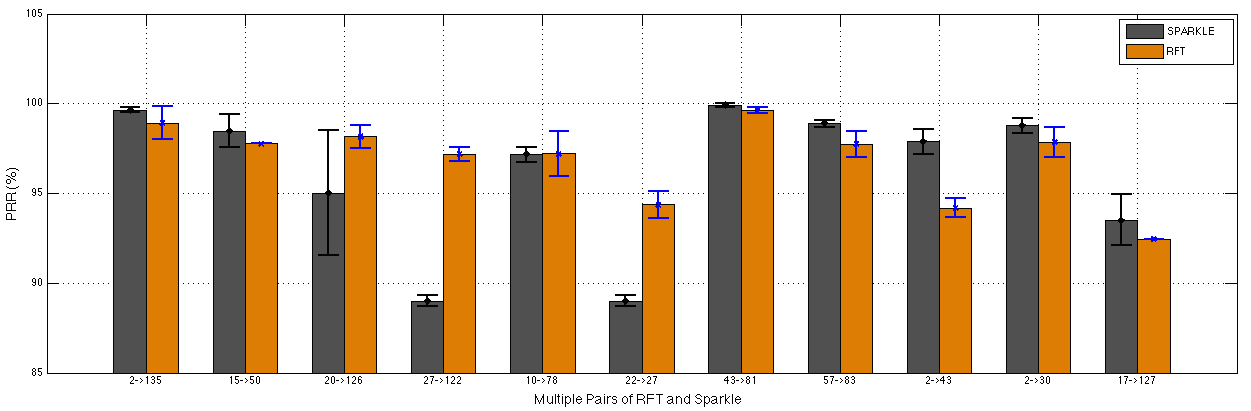
\includegraphics[width=16cm]{groupbar_prr_rft_spkl.png}
\caption{The Packet Reception Rate of multiple pairs in Sparkle vs. RFT.}
\label{fig:PRRcompare}
\end{figure*}

\subsubsection{Scenarios}
To test the two protocol performance, we use all the available nodes of the testbed around 100 nodes and choose several nodes in different floors as sources and destinations. We consider the link setup and time synchronisation processes belong to the control overhead, not just only consider the link setup as Sparkle paper mentions. Energest provided by Contiki has been used to measure the radio-on time for controlling and data transmission. To compute the energy consumption in high accuracy, we consider the different current level of listen mode and transmission mode with default transmission power level index as shown in the Tmote Sky data sheet. Multiplied by the current of transmission or reception and the default voltage with the radio-on time, the precise energy consumption can be computed. %Since the network is relative large and the destination is even located at two floors below in some cases, the energy usage for the management have much proportion of the whole energy consumption.
\begin{figure*}
\centering
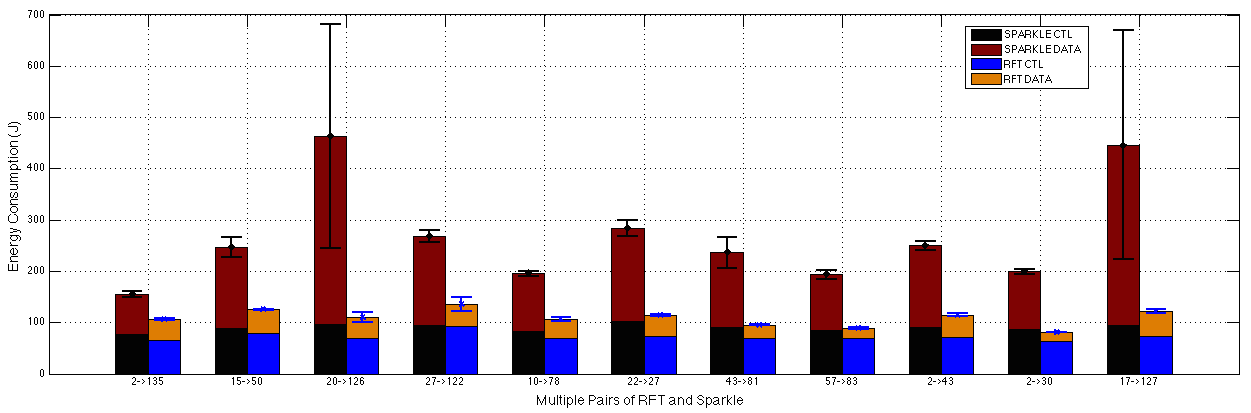
\includegraphics[width=16cm]{stackbar_energy_rft_spkl.png}
\caption{The average energy consumption of multiple pairs in Sparkle vs. RFT. The energy is the sum of all the nodes consumed during one hour experiment. ALL is the whole energy consumption, DATA stand for energy usage of data transmission.}
\label{fig:Energycompare}
\end{figure*}
\subsubsection{Results}
RFT has the relative similar PRR with Sparkle but is more stable, shown in Fig.~\ref{fig:PRRcompare}. We separate the energy usage into two parts as shown in Fig.~\ref{fig:Energycompare}. RFT has tremendous energy savings compared to Sparkle. The energy usage of Sparkle have relative high variation since it performs modes switches, including flooding, one hundred paths and two most frequent paths. The data traffic of Sparkle dominates the energy consumption, as mentioned in Sparkle, however Sparkle may flood or use over 20 nodes for the data transmission. The data transmission of Sparkle consumes averagely 4.8 times and maximum 11.8 times energy than RFT. On the contrast, our protocol has low deviation of energy consumption and maintains the high energy efficiency and end-to-end reliability. 

%\hfill mds
 
%\hfill January 11, 2007

%\subsection{Subsection Heading Here}
%Subsection text here.
%
%
%\subsubsection{Subsubsection Heading Here}
%Subsubsection text here.


% An example of a floating figure using the graphicx package.
% Note that \label must occur AFTER (or within) \caption.
% For figures, \caption should occur after the \includegraphics.
% Note that IEEEtran v1.7 and later has special internal code that
% is designed to preserve the operation of \label within \caption
% even when the captionsoff option is in effect. However, because
% of issues like this, it may be the safest practice to put all your
% \label just after \caption rather than within \caption{}.
%
% Reminder: the "draftcls" or "draftclsnofoot", not "draft", class
% option should be used if it is desired that the figures are to be
% displayed while in draft mode.
%
%\begin{figure}[!t]
%\centering
%\includegraphics[width=2.5in]{myfigure}
% where an .eps filename suffix will be assumed under latex, 
% and a .pdf suffix will be assumed for pdflatex; or what has been declared
% via \DeclareGraphicsExtensions.
%\caption{Simulation Results}
%\label{fig_sim}
%\end{figure}

% Note that IEEE typically puts floats only at the top, even when this
% results in a large percentage of a column being occupied by floats.


% An example of a double column floating figure using two subfigures.
% (The subfig.sty package must be loaded for this to work.)
% The subfigure \label commands are set within each subfloat command, the
% \label for the overall figure must come after \caption.
% \hfil must be used as a separator to get equal spacing.
% The subfigure.sty package works much the same way, except \subfigure is
% used instead of \subfloat.
%
%\begin{figure*}[!t]
%\centerline{\subfloat[Case I]\includegraphics[width=2.5in]{subfigcase1}%
%\label{fig_first_case}}
%\hfil
%\subfloat[Case II]{\includegraphics[width=2.5in]{subfigcase2}%
%\label{fig_second_case}}}
%\caption{Simulation results}
%\label{fig_sim}
%\end{figure*}
%
% Note that often IEEE papers with subfigures do not employ subfigure
% captions (using the optional argument to \subfloat), but instead will
% reference/describe all of them (a), (b), etc., within the main caption.


% An example of a floating table. Note that, for IEEE style tables, the 
% \caption command should come BEFORE the table. Table text will default to
% \footnotesize as IEEE normally uses this smaller font for tables.
% The \label must come after \caption as always.
%
%\begin{table}[!t]
%% increase table row spacing, adjust to taste
%\renewcommand{\arraystretch}{1.3}
% if using array.sty, it might be a good idea to tweak the value of
% \extrarowheight as needed to properly center the text within the cells
%\caption{An Example of a Table}
%\label{table_example}
%\centering
%% Some packages, such as MDW tools, offer better commands for making tables
%% than the plain LaTeX2e tabular which is used here.
%\begin{tabular}{|c||c|}
%\hline
%One & Two\\
%\hline
%Three & Four\\
%\hline
%\end{tabular}
%\end{table}


% Note that IEEE does not put floats in the very first column - or typically
% anywhere on the first page for that matter. Also, in-text middle ("here")
% positioning is not used. Most IEEE journals/conferences use top floats
% exclusively. Note that, LaTeX2e, unlike IEEE journals/conferences, places
% footnotes above bottom floats. This can be corrected via the \fnbelowfloat
% command of the stfloats package.



\section{Conclusion}
We present RFT protocol, a lightweight and fast communication protocol for point-to-point traffic in low-power wireless sensor network. Recent works from academia have shown the feasibility and benefits of concurrent transmission applied for the point-to-point data traffic.  Despite with diversified topology control methods, existing state-of-art approaches utilise many redundant nodes for the high reliability and cost the energy wastage. RFT identifies the reliable relay nodes and neighbours of relays as the concurrent transmitters to reinforce the reliability of links. With the benefits of constructive interference, the consolidated paths gain higher end-to-end reliability and energy efficiency. Results from the real-world testbed show RFT averagely reduces 75.6\% energy consumption for data transmission with the high end-to-end reliability across all scenarios. %Low power wireless bus and Chaos offer high yield and flexible data traffic, low duty cycles and high end-to-end packet reception ratio. However the scenarios like controlling and multimedia information need the reliable and flexible point-to-point data communication pattern. CXFS and Sparkle introduce the topology control theory for point-to-point data traffic, and reduce impressive energy wastage by turning off radio of the unhelpful nodes. But there still exist the fragile link like the short slab of the bucket. And the additional neighbours that keep good connections with more than 2 relays are to selected precisely and effectively to reinforce these weak points.




% conference papers do not normally have an appendix


% use section* for acknowledgement
\section*{Acknowledgment}


We would like to thank the anonymous reviewers.





% trigger a \newpage just before the given reference
% number - used to balance the columns on the last page
% adjust value as needed - may need to be readjusted if
% the document is modified later
%\IEEEtriggeratref{8}
% The "triggered" command can be changed if desired:
%\IEEEtriggercmd{\enlargethispage{-5in}}

% references section

% can use a bibliography generated by BibTeX as a .bbl file
% BibTeX documentation can be easily obtained at:
% http://www.ctan.org/tex-archive/biblio/bibtex/contrib/doc/
% The IEEEtran BibTeX style support page is at:
% http://www.michaelshell.org/tex/ieeetran/bibtex/
\bibliographystyle{IEEEtran}
% argument is your BibTeX string definitions and bibliography database(s)
\bibliography{rft}
%
% <OR> manually copy in the resultant .bbl file
% set second argument of \begin to the number of references
% (used to reserve space for the reference number labels box)
%\begin{thebibliography}{1}
%
%\bibitem{IEEEhowto:kopka}
%H.~Kopka and P.~W. Daly, \emph{A Guide to \LaTeX}, 3rd~ed.\hskip 1em plus
%  0.5em minus 0.4em\relax Harlow, England: Addison-Wesley, 1999.
%
%\end{thebibliography}




% that's all folks
\end{document}


